	\section{不定方程}
	未知数个数多于方程个数的方程(或方程组)称为不定方程(或不定方程组), 初等数论中仅讨论未知数取值为整数的情形. 这一单元主要讨论不定方程的求解问题中涉及的一些基本方法.

	不定方程溯源极古, 早在 1700 多年前, 古希腊数学家丢番图(Diophantus)就对不定方程做过许多研究, 不定方程甚至被称为丢番图方程. 许多不定方程问题的解决十分困难, 是对人类智力的一种挑战, 例如历时 358 年方获解决的费马大定理就曾吸引无数优秀数学家为之付出毕生的精力. 面对挑战, 人类表现出了极大的决心, 毅力和杰出的智慧.

	\section{一次不定方程(组)}
	依未知数的次数可对不定方程分类, 其中最简单的是一次不定方程. \\
	设 $k \geqslant 2$ 为整数, 我们称方程
\begin{align*}
		a_{1} x_{1}+a_{2} x_{2}+\cdots+a_{k} x_{k}=c
	\end{align*}

	为一次不定方程, 其中 $a_{1} ,  a_{2} ,  \cdots ,  a_{k} ,  c$ 均为整数, 且 $a_{1} ,  a_{2} ,  \cdots ,  a_{k}$ 都不为零.

	并非每一个一次不定方程都会有整数解, 一个很显然的必要条件是:  $\left(a_{1}, a_{2}, \cdots, a_{k}\right) \mid c$ . 事实上, 这个条件也是充分的. 我们重点讨论两个变量的不定方程
\begin{align*}
		a x+b y=c
	\end{align*}

	其中 $a ,  b ,  c$ 为整数, 且 $a ,  b$ 都不为零. \\
	定理1 不定方程(2)有整数解的充要条件是 $(a, b) \mid c$ . \\
	证明 必要性是显然的, 而充分性可由贝祖定理得到. \\
	事实上, 由贝祖定理, 知存在整数 $x_{0} ,  y_{0}$ , 使得 $a x_{0}+b y_{0}=(a, b)$ . 设 $c=(a, b) c_{1}$ , 则 $\left(c_{1} x_{0}, c_{1} y_{0}\right)$ 是(2)的解, 充分性获证.

	定理2 设不定方程(2)有整数解 $\left(x_{0}, y_{0}\right)$ , 则(2)的所有整数解为
\begin{align*}
		\left\{\begin{array}{l}
			       x=x_{0}+\frac{b}{(a, b)} t, \\
			       y=y_{0}-\frac{a}{(a, b)} t .
		       \end{array}(t \text { 为整数 })\right.
	\end{align*}

	证明 设 $(x, y)$ 是(2)的一组整数解, 结合 $\left(x_{0}, y_{0}\right)$ 为(2)的解, 可知
\begin{align*}
		\left\{\begin{array}{l}
			       a x+b y=c \\
			       a x_{0}+b y_{0}=c
		       \end{array}\right.
	\end{align*}

	于是
\begin{align*}
		a\left(x-x_{0}\right)+b\left(y-y_{0}\right)=0
	\end{align*}

	即
\begin{align*}
		a\left(x-x_{0}\right)=b\left(y_{0}-y\right)
	\end{align*}

	故
\begin{align*}
		b \mid a\left(x-x_{0}\right)
	\end{align*}

	因此
\begin{align*}
		\left.\frac{b}{(a, b)} \right\rvert\, x-x_{0}
	\end{align*}

	可设
\begin{align*}
		x-x_{0}=\frac{b}{(a, b)} t
	\end{align*}

	则
\begin{align*}
		y-y_{0}=-\frac{a}{(a, b)} t
	\end{align*}

	其中 $t$ 为整数, 这表明方程(2)的解具有形式(3).\\
	反过来, 由(3)决定的整数组( $x, y$ )是方程(2)的解可以直接代入(2)验证得到.

	所以, 定理 2 成立. \\
	说明 由(3)决定的整数组 $(x, y)$ 称为(2)的通解, 而 $\left(x_{0}, y_{0}\right)$ 为(2)的特解.定理 2 也表明为求(2)的通解只需先求出(2)的一个特解, 而特解可由辗转相除的方法逆算得到, 因此(2)的所有解有通法求出.

	其余的一次不定方程或方程组都可以转化为求解二元一次不定方程. \\
	例1 求不定方程
\begin{align*}
		7 x+19 y=2012
	\end{align*}

	的正整数解的组数.\\
	解 先求出(1)的一个特解.
\begin{align*}
		x=\frac{1}{7}(2012-19 y)=287-3 y+\frac{1}{7}(3+2 y)
	\end{align*}

	故 $\frac{1}{7}(3+2 y)$ 为整数, 取 $y_{0}=2$, 则 $x_{0}=282$.\\
	利用定理 2 的结论, 方程(1)的通解为
\begin{align*}
		\left\{\begin{array}{l}
			       x=282-19 t, \\
			       y=2+7 t .
		       \end{array}\right.
	\end{align*}

	结合 $x>0, y>0$ 及 $t$ 为整数, 可解得 $0 \leqslant t \leqslant 14$.\\
	所以, 方程 (1) 共有 15 组正整数解.\\
	例2 设正整数 $a ,  b$ 互素. 证明: 不定方程
\begin{align*}
		a x+b y=a b-a-b
	\end{align*}

	没有非负整数解.\\
	证明 若存在非负整数对 $\left(x_{0}, y_{0}\right)$ 满足 (1), 则
\begin{align*}
		a\left(x_{0}+1\right)+b\left(y_{0}+1\right)=a b
	\end{align*}

	那么, 应有
\begin{align*}
		a \mid b\left(y_{0}+1\right)
	\end{align*}

	又
\begin{align*}
		(a, b)=1
	\end{align*}

	故
\begin{align*}
		a \mid y_{0}+1
	\end{align*}

	而 $a$ 与 $y_{0}+1$ 都是正整数, 故 $a \leqslant y_{0}+1$.\\
	同理可证: $b \mid x_{0}+1$, 进而 $b \leqslant x_{0}+1$. 但这时, (2)的左边 $\geqslant a b+b a=$ $2 a b>$ (2) 的右边, 矛盾.

	所以, (1)没有非负整数解.\\
	例3 设正整数 $a ,  b$ 互素, 而正整数 $c$ 大于 $a b-a-b$. 证明: 不定方程
\begin{align*}
		a x+b y=c
	\end{align*}

	有非负整数解.\\
	证明 设(1)的通解为
\begin{align*}
		\left\{\begin{array}{l}
			       x=x_{0}+b t, \\
			       y=y_{0}-a t
		       \end{array}(t \text { 为整数 })\right.
	\end{align*}

	其中 $\left(x_{0}, y_{0}\right)$ 为(1)的特解.\\
	这样, 通过调节 $t$ 的值 (对 $x_{0}$ 作加上 $b$ 或减去 $b$ 的操作) 可找到(1)的一个解 $\left(x_{1}, y_{1}\right)$ , 使得 $0 \leqslant x_{1} \leqslant b-1$ , 则
\begin{align*}
		b y_{1}=c-a x_{1}>a b-a-b-a x_{1} \geqslant a b-a-b-a(b-1)=-b
	\end{align*}

	故
\begin{align*}
		y_{1}>-1,
	\end{align*}

	即
\begin{align*}
		y_{1} \geqslant 0
	\end{align*}

	这表明 $\left(x_{1}, y_{1}\right)$ 是(1)的非负整数解, 命题获证. \\
	说明 上面的两个例子得到的结论给出了使得(1)有非负整数解的条件, 说明了只要 $c$ 充分大(例如 $c \geqslant c_{0}$ 时), (1)就有非负整数解, 并求出了 $c_{0}$ 的最小值(这个最小值为 $a b-a-b+1$ ). 这是一个有趣而富有挑战性的问题, 当变量个数不小于 3 时, $c_{0}$ 的最小值还没有找到.

	例 4 求不定方程
\begin{align*}
		x+2 y+3 z=2012
	\end{align*}

	的正整数解的组数.\\
	解 设 $(x, y, z)$ 为(1)的正整数解, 则 $3 z \leqslant 2009$ , 即 $1 \leqslant z \leqslant 669$ , 分别可得
\begin{align*}
		x+2 y=2009,2006, \cdots, 5
	\end{align*}

	对应地, $y$ 的取值范围分别是\begin{align}
		 & 1 \leqslant y \leqslant 1004,1 \leqslant y \leqslant 1002,1 \leqslant y \leqslant 1001 \\
		 & 1 \leqslant y \leqslant 999, \cdots, 1 \leqslant y \leqslant 2
	\end{align}

	由于当 $y ,  z$ 确定后,  $x$ 的值唯一确定, 所以(1)的正整数解共有\begin{align}
		  & (1004+1002)+(1001+999)+\cdots+(5+3)+2 \\
		= & 2006+2000+\cdots+8+2                  \\
		= & \frac{1}{2}(2006+2) \times 335=336340
	\end{align}

	综上可知, 共有 336340 组正整数解. \\
	例 5 求所有的正整数数组 $\left(a_{1}, a_{2}, \cdots, a_{n}\right)$ , 使得
\begin{align*}
		\left\{\begin{array}{l}
			       a_{1} \leqslant a_{2} \leqslant \cdots \leqslant a_{n} \\
			       a_{1}+a_{2}+\cdots+a_{n}=26                            \\
			       a_{1}^{2}+a_{2}^{2}+\cdots+a_{n}^{2}=62                \\
			       a_{1}^{3}+a_{2}^{3}+\cdots+a_{n}^{3}=164
		       \end{array}\right.
	\end{align*}

	解 由 $a_{i}$ 都是正整数, 而 $6^{3}=216>164$ , 知每个 $a_{i}$ 都不大于 5 . 我们设 $a_{1}, a_{2}, \cdots, a_{n}$ 中 $1,2,3,4,5$ 的个数分别为 $x_{1}, x_{2}, x_{3}, x_{4}, x_{5}$ , 则
\begin{align*}
		\left\{\begin{array}{l}
			       x_{1}+x_{2}+x_{3}+x_{4}+x_{5}=n            \\
			       x_{1}+2 x_{2}+3 x_{3}+4 x_{4}+5 x_{5}=26   \\
			       x_{1}+4 x_{2}+9 x_{3}+16 x_{4}+25 x_{5}=62 \\
			       x_{1}+8 x_{2}+27 x_{3}+64 x_{4}+125 x_{5}=164
		       \end{array}\right.
	\end{align*}

	其中 $x_{1}, x_{2}, x_{3}, x_{4}, x_{5}$ 都是非负整数.\\
	先确定 $x_{1}, x_{2}, \cdots, x_{5}$ 的值, 这等价于求一个不定方程组的非负整数解. \\
	由(4)知 $x_{5} \leqslant 1$, 若 $x_{5}=1$, 则(3), (4)变为
\begin{align*}
		\left\{\begin{array}{l}
			       x_{1}+4 x_{2}+9 x_{3}+16 x_{4}=37 \\
			       x_{1}+8 x_{2}+27 x_{3}+64 x_{4}=39
		       \end{array}\right.
	\end{align*}

	由 (6) - (5) 得
\begin{align*}
		4 x_{2}+18 x_{3}+48 x_{4}=2
	\end{align*}

	这在 $x_{2} ,  x_{3} ,  x_{4}$ 为非负整数时不能成立, 所以
\begin{align*}
		x_{5}=0
	\end{align*}

	又由 (3) - (2) 得 $2 x_{2}+6 x_{3}+12 x_{4}=36$ ,

	即
\begin{align*}
		x_{2}+3 x_{3}+6 x_{4}=18
	\end{align*}

	由 (4) 一 (2) 得
\begin{align*}
		x_{2}+4 x_{3}+10 x_{4}=23
	\end{align*}

	再由 (8) - (7) 得 $\quad x_{3}+4 x_{4}=5$,\\
	故
\begin{align*}
		\left(x_{3}, x_{4}\right)=(5,0),(1,1)
	\end{align*}

	进而可得
\begin{align*}
		\left(x_{1}, x_{2}, x_{3}, x_{4}\right)=(5,3,5,0),(1,9,1,1)
	\end{align*}

	利用上述结论, 可知\begin{align}
		  & \left(a_{1}, a_{2}, \cdots, a_{n}\right) \\
		= & (1,1,1,1,1,2,2,2,3,3,3,3,3)              \\
		  & (1,2,2,2,2,2,2,2,2,2,3,4)
	\end{align}

	说明 上述两例中都用到了不等式估计的方法, 并没有从不定方程(组)的通解出发来处理, 解题过程中把握了问题的特点, 因此较快地得到了解答.

	例6 将所有分母不大于 99 的最简分数从小到大排列, 求与 $\frac{17}{76}$ 相邻的两个数.

	解 设 $\frac{q}{p}$ 与 $\frac{n}{m}$ 是与 $\frac{17}{76}$ 相邻的两个数, 且
\begin{align*}
		\frac{q}{p}<\frac{17}{76}<\frac{n}{m}
	\end{align*}

	其中 $p ,  q ,  m ,  n$ 为正整数, 则

	于是\begin{align}
		 & 17 p-76 q>0           \\
		 & 17 p-76 q \geqslant 1
	\end{align}

	先考虑 $17 p-76 q=1$ 中满足 $p \leqslant 99$ 且使 $p$ 最大的正整数解. 为此需先求它的一个特解, 利用
\begin{align*}
		p=\frac{1}{17}(76 q+1)=4 q+\frac{1}{17}(8 q+1)
	\end{align*}

	可得一个特解 $(p, q)=(9,2)$, 于是此不定方程的通解为
\begin{align*}
		(p, q)=(9+76 t, 2+17 t)
	\end{align*}\\
$t$ 为整数. 这时在条件 $p \leqslant 99$ 下, $p$ 最大为 85 , 此时 $q=19$ . \\
	另一方面, 由
\begin{align*}
		\frac{17}{76}-\frac{q}{p}=\frac{17 p-76 q}{76 p}
	\end{align*}

	可知, 若 $17 p-76 q \geqslant 2$, 则
\begin{align*}
		\frac{17}{76}-\frac{q}{p} \geqslant \frac{2}{76 p}=\frac{1}{38 p} \geqslant \frac{1}{38 \times 99}>\frac{1}{76 \times 85}=\frac{17}{76}-\frac{19}{85}
	\end{align*}

	所以, 在所给条件下, 比 $\frac{17}{76}$ 小且最接近它的数为 $\frac{19}{85}$ . \\
	类似讨论, 可知 $\frac{n}{m}=\frac{15}{67}$ . \\
	综上, 这些分数的排列中与 $\frac{17}{76}$ 相邻的两个数是 $\frac{19}{85}$ 和 $\frac{15}{67}$.\\
	说明 题中利用正整数不小于 1 这个显然的事实, 转为求一次不定方程的正整数解是关键.

	\section{2 不定方程的常用解法}
	对于高次不定方程, 求出其通解然后再讨论有时是不现实的, 因为我们甚至还没有找到判别一个高次不定方程是否有解的统一方法, 当然要求出通解就更难了. 或许正是因为没有统一的方法来处理高次不定方程, 对具体的

	问题往往有许多方法来处理, 并且每一种方法都表现出一定的创造性, 所以, 高次不定方程的问题频繁地在数学竞赛中出现.

	当然, 结合整除与同余的一些理论, 求解高次不定方程也有一些常见的处理思路和解决办法.

	\section{一, 因式分解法}
	将方程的一边变为常数, 而含字母的一边可以进行因式分解, 这样对常数进行素因数分解后, 对比方程两边, 考察各因式的每种取值情况就可将不定方程变为若干个方程组去求解. 这就是因式分解法处理不定方程的基本思路.

	例 1 求方程
\begin{align*}
		x y-10(x+y)=1
	\end{align*}

	的整数解.\\
	解 利用十字相乘, 可将(1)变形为
\begin{align*}
		(x-10)(y-10)=101
	\end{align*}

	而 101 为素数, 故\begin{align}
		  & (x-10, y-10)                        \\
		= & (1,101),(101,1),(-1,-101),(-101,-1)
	\end{align}

	分别求解, 得方程的整数解为
\begin{align*}
		(x, y)=(11,111),(111,11),(9,-91),(-91,9)
	\end{align*}

	例 2 是否存在整数 $x ,  y ,  z$, 使得
\begin{align*}
		x^{4}+y^{4}+z^{4}=2 x^{2} y^{2}+2 y^{2} z^{2}+2 z^{2} x^{2}+24 ?
	\end{align*}

	解 若存在整数 $x ,  y ,  z$ 满足条件, 则\begin{align}
		-24 & =2 x^{2} y^{2}+2 y^{2} z^{2}+2 z^{2} x^{2}-\left(x^{4}+y^{4}+z^{4}\right)          \\
		    & =-\left(x^{2}+y^{2}\right)^{2}+2\left(x^{2}+y^{2}\right) z^{2}-z^{4}+4 x^{2} y^{2} \\
		    & =-\left(x^{2}+y^{2}-z^{2}\right)^{2}+4 x^{2} y^{2}                                 \\
		    & =\left(2 x y+x^{2}+y^{2}-z^{2}\right)\left(2 x y-x^{2}-y^{2}+z^{2}\right)          \\
		    & =\left((x+y)^{2}-z^{2}\right)\left(z^{2}-(x-y)^{2}\right)                          \\
		    & =(x+y+z)(x+y-z)(z+x-y)(y+z-x)
	\end{align}

	这要求 -24 能表示为 4 个整数 $x+y+z, x+y-z, z+x-y, y+z-x$ 的乘积的形式, 而这 4 个数中任意两个数之差都为偶数, 故这 4 个数具有相同的

	奇偶性, 由 -24 为偶数, 知它们都是偶数, 但这要求 $2^{4} \mid 24$, 矛盾.\\
	所以,不存在符合要求的整数.\\
	说明 熟悉海伦公式的读者可以一眼看穿问题的本质. 事实上, $S_{\triangle A B C}=$ $\frac{1}{4} \sqrt{(a+b+c)(a+b-c)(b+c-a)(c+a-b)}$, 其中 $a ,  b ,  c$ 为 $\triangle A B C$ 的三边长, 这就是海伦公式. 根号里面的式子展开后就是 $2 a^{2} b^{2}+2 b^{2} c^{2}+2 c^{2} a^{2}-$ $a^{4}-b^{4}-c^{4}$ .

	例 3 求所有的正整数对 $(m, n)$, 使得
\begin{align*}
		n^{5}+n^{4}=7^{m}-1
	\end{align*}

	解 将(1)移项后作因式分解, 得\begin{align}
		7^{m} & =n^{5}+n^{4}+1=n^{5}+n^{4}+n^{3}-\left(n^{3}-1\right)    \\
		      & =n^{3}\left(n^{2}+n+1\right)-(n-1)\left(n^{2}+n+1\right) \\
		      & =\left(n^{3}-n+1\right)\left(n^{2}+n+1\right)
	\end{align}

	由(1)知 $n>1$ , 而 $n=2$ 时, 可得 $m=2$ . \\
	下面考虑 $n>2$ 的情形, 我们先看(2)式右边两个式子的最大公因数.\begin{align}
		  & \left(n^{3}-n+1, n^{2}+n+1\right)=\left(n^{3}-n+1-\left(n^{2}+n+1\right)(n-1), n^{2}+n+1\right) \\
		= & \left(-n+2, n^{2}+n+1\right)=\left(-n+2, n^{2}+n+1+(-n+2)(n+3)\right)                           \\
		= & (-n+2,7)
	\end{align}

	故 $\left(n^{3}-n+1, n^{2}+n+1\right) \mid 7$.\\
	结合(2)式知 $n^{3}-n+1$ 与 $n^{2}+n+1$ 都是 7 的幂次, 而它们在 $n \geqslant 3$ 时, 都大于 7 , 这导致 $7^{2} \mid\left(n^{3}-n+1, n^{2}+n+1\right)$ , 与前所得矛盾.

	综上可知, 只有 $(m, n)=(2,2)$ 符合要求.\\
	说明 对(1)式变形后, 所得(2)式两边符合因式分解方法解不定方程的套路, 但 $7^{m}$ 并不是一个常数, 这里需要有另外的方法来处理才能继续下去. 活学活用方能攻城拔寨.

	\section{二, 配方法}
	配方是代数变形中的常见方法, 在处理不定方程的问题时还可综合利用完全平方数的特性, 因此配方法在求解不定方程时大有用武之地.

	例 4 求不定方程 $3 x^{2}-4 x y+3 y^{2}=35$ 的全部整数解. \\
	解 对方程两边都乘以 3 , 配方后即得
\begin{align*}
		(3 x-2 y)^{2}+5 y^{2}=105
	\end{align*}

	由(1)式得\\
	所以
\begin{align*}
		5 y^{2} \leqslant 105
	\end{align*}
\begin{align*}
		|y| \leqslant 4
	\end{align*}

	当 $|y|=4$ 时, $|3 x-2 y|=5$ , 此时原方程的解为
\begin{align*}
		(x, y)=(1,4),(-1,-4)
	\end{align*}

	当 $|y|=1$ 时, $|3 x-2 y|=10$ , 此时原方程的解为
\begin{align*}
		(x, y)=(4,1),(-4,-1)
	\end{align*}

	当 $|y|=0,2,3$ 时, $(3 x-2 y)^{2}$ 分别为 $105,85,60$. 此时, 所得的方程组显然无整数解.

	上面的讨论表明, 原方程有 4 组解: 
\begin{align*}
		(x, y)=(4,1),(1,4),(-4,-1),(-1,-4)
	\end{align*}

	例 5 求方程 $x^{2}+x=y^{4}+y^{3}+y^{2}+y$ 的整数解. \\
	解 同上例, 对方程两边同乘以 4 , 并对左边进行配方, 得
\begin{align*}
		(2 x+1)^{2}=4\left(y^{4}+y^{3}+y^{2}+y\right)+1
	\end{align*}

	下面对(1)式右端进行估计. 由于\begin{align}
		  & 4\left(y^{4}+y^{3}+y^{2}+y\right)+1       \\
		= & \left(2 y^{2}+y+1\right)^{2}-y^{2}+2 y    \\
		= & \left(2 y^{2}+y\right)^{2}+3 y^{2}+4 y+1,
	\end{align}

	从而, 当 $y>2$ 或 $y<-1$ 时, 有
\begin{align*}
		\left(2 y^{2}+y\right)^{2}<(2 x+1)^{2}<\left(2 y^{2}+y+1\right)^{2}
	\end{align*}

	由于 $2 y^{2}+y$ 与 $2 y^{2}+y+1$ 是两个连续的整数, 它们的平方之间不会含有完全平方数, 故上式不成立.

	因此只需考虑当 $-1 \leqslant y \leqslant 2$ 时方程的解, 这是平凡的, 容易得到原方程的全部整数解是
\begin{align*}
		(x, y)=(0,-1),(-1,-1),(0,0),(-1,0),(-6,2),(5,2)
	\end{align*}

	例 6 求所有的正整数 $n \geqslant 2$, 使得不定方程组
\begin{align*}
		\left\{\begin{array}{c}
			       x_{1}^{2}+x_{2}^{2}+50=16 x_{1}+12 x_{2}     \\
			       x_{2}^{2}+x_{3}^{2}+50=16 x_{2}+12 x_{3}     \\
			       \cdots                                       \\
			       x_{n-1}^{2}+x_{n}^{2}+50=16 x_{n-1}+12 x_{n} \\
			       x_{n}^{2}+x_{1}^{2}+50=16 x_{n}+12 x_{1}
		       \end{array}\right.
	\end{align*}

	有整数解.\\
	解 移项后配方, 方程组变形为
\begin{align*}
		\left\{\begin{array}{c}
			       \left(x_{1}-8\right)^{2}+\left(x_{2}-6\right)^{2}=50   \\
			       \left(x_{2}-8\right)^{2}+\left(x_{3}-6\right)^{2}=50   \\
			       \cdots                                                 \\
			       \left(x_{n-1}-8\right)^{2}+\left(x_{n}-6\right)^{2}=50 \\
			       \left(x_{n}-8\right)^{2}+\left(x_{1}-6\right)^{2}=50
		       \end{array}\right.
	\end{align*}

	由于 50 表示为两个正整数的平方和只有两种: $50=1^{2}+7^{2}=5^{2}+5^{2}$, 所以,由(1)知 $\left|x_{2}-6\right|=1 ,  5$ 或 7,而由(2)知 $\left|x_{2}-8\right|=1 ,  5$ 或 7, 从而 $x_{2}=1$ ,  7 或 13 .

	进一步,可知对每个 $1 \leqslant i \leqslant n$ , 都有 $x_{i}=1,7$ 或 13 , 依 $x_{1}=1 ,  7 ,  13$ , 分三种情况讨论.

	若 $x_{1}=1$,则由(1)知 $x_{2}=7$, 再由 (2)知 $x_{3}=13$, 依次往下递推, 可知当 $k \equiv 1(\bmod 3)$ 时,  $x_{k}=1$ ; 当 $k \equiv 2(\bmod 3)$ 时,  $x_{k}=7$ ; 当 $k \equiv 0(\bmod 3)$ 时,  $x_{k}=13$. 所以, 由第 (2) 式, 知当且仅当 $n+1 \equiv 1(\bmod 3)$ 时, 原方程组有整数解, 即当且仅当 $3 \mid n$ 时, $n$ 符合要求.

	对另外两种情况 $x_{1}=7$ 和 $x_{1}=13$ 同样讨论, 得到的条件是一样的.\\
	综上可知, 满足条件的 $n$ 是所有 3 的倍数. \\
	说明 进一步讨论可知, 当 $3 \mid n$ 时, 方程组恰有 3 组整数解.

	\section{三, 不等式估计}
	利用不等式的知识, 先确定不定方程中的某个字母的范围, 然后逐个枚举得到所有解, 这个方法称为不等式估计, 它也是我们处理不定方程的常见方法. 当然, 如果能够恰当地利用字母的对称性等, 那么作不等式估计时会简洁很多.

	例 7 求不定方程 $x^{3}-y^{3}=x y+61$ 的正整数解.\\
	解 设 $(x, y)$ 为方程的正整数解, 则 $x>y$. 设 $x=y+d$, 则 $d$ 为正整数, 且\begin{align}
		(y+d) y+61 & =(y+d)^{3}-y^{3}           \\
		           & =3 d y^{2}+3 y d^{2}+d^{3}
	\end{align}

	即有
\begin{align*}
		(3 d-1) y^{2}+d(3 d-1) y+d^{3}=61
	\end{align*}

	故
\begin{align*}
		d^{3}<61
	\end{align*}

	于是
\begin{align*}
		d \leqslant 3
	\end{align*}

	分别令 $d=1 ,  2 ,  3$ 代入, 得\begin{align}
		 & 2 y^{2}+2 y+1=61   \\
		 & 5 y^{2}+10 y+8=61  \\
		 & 8 y^{2}+24 y+27=61
	\end{align}

	只有第一个方程有整数解, 并由 $y$ 为正整数知 $y=5$, 进而 $x=6$.\\
	所以, 原方程只有一组正整数解 $(x, y)=(6,5)$.\\
	例 8 求所有的正整数 $a ,  b$, 使得
\begin{align*}
		4^{a}+4 a^{2}+4=b^{2}
	\end{align*}

	解 若 $(a ,  b)$ 是满足(1) 的正整数数对, 则 $b^{2}$ 为偶数, 且 $b^{2}>4^{a}$, 从而 $b$ 为偶数, 且 $b>2^{a}$, 故 $b \geqslant 2^{a}+2$. 于是
\begin{align*}
		4^{a}+4 a^{2}+4=b^{2} \geqslant\left(2^{a}+2\right)^{2}=4^{a}+4 \cdot 2^{a}+4
	\end{align*}

	知 $a^{2} \geqslant 2^{a}$, 可得 $a \leqslant 4$ (对 $a$ 归纳可证: 当 $a \geqslant 5$ 时, 有 $a^{2}<2^{a}$ ).\\
	分别就 $a=1,2,3,4$ 代入 (1) 式, 可得方程的所有正整数解为 $(a, b)=$ $(2,6)$ 或 $(4,18)$.

	例 9 求所有的正整数数组 $(a, b, c, x, y, z)$, 使得
\begin{align*}
		\left\{\begin{array}{l}
			       a+b+c=x y z \\
			       x+y+z=a b c
		       \end{array}\right.
	\end{align*}

	这里 $a \geqslant b \geqslant c, x \geqslant y \geqslant z$.\\
	解 由对称性, 我们只需考虑 $x \geqslant a$ 的情形. 这时
\begin{align*}
		x y z=a+b+c \leqslant 3 a \leqslant 3 x
	\end{align*}

	故
\begin{align*}
		y z \leqslant 3
	\end{align*}

	于是
\begin{align*}
		(y, z)=(1,1),(2,1),(3,1)
	\end{align*}

	当 $(y, z)=(1,1)$ 时, $a+b+c=x$ 且 $x+2=a b c$, 于是
\begin{align*}
		a b c=a+b+c+2 .
	\end{align*}

	若 $c \geqslant 2$, 则
\begin{align*}
		a+b+c+2 \leqslant 3 a+2 \leqslant 4 a \leqslant a b c,
	\end{align*}

	等号当且仅当 $a=b=c=2$ 时成立.\\
	若 $c=1$, 则
\begin{align*}
		a b=a+b+3
	\end{align*}

	即
\begin{align*}
		(a-1)(b-1)=4
	\end{align*}

	得
\begin{align*}
		(a, b)=(5,2),(3,3)
	\end{align*}

	当 $(y, z)=(2,1)$ 时, $2 a b c=2 x+6=a+b+c+6$ , 与上述类似讨论可知 $c=1$ , 进而

	得
\begin{align*}
		\begin{gathered}
			(2 a-1)(2 b-1)=15 \\
			(a, b)=(3,2)
		\end{gathered}
	\end{align*}

	当 $(y, z)=(3,1)$ 时, $3 a b c=3 x+12=a+b+c+12$, 类似可知,此时无解.

	综上所述, 可知\begin{align}
		  & (a, b, c, x, y, z)                        \\
		= & (2,2,2,6,1,1),(5,2,1,8,1,1),(3,3,1,7,1,1) \\
		  & (3,2,1,3,2,1),(6,1,1,2,2,2),(8,1,1,5,2,1) \\
		  & (7,1,1,3,3,1)
	\end{align}

	说明 此题中如果没有条件 $a \geqslant b \geqslant c$ 和 $x \geqslant y \geqslant z$ , 也需要利用对称性作出这样的假设后再处理, 解题中利用对称性假设 $x \geqslant a$ 是巧妙的, 这样问题就转化为只有 3 种情况而便于处理了.

	\section{四, 同余方法}
	若不定方程 $F\left(x_{1}, x_{2}, \cdots, x_{n}\right)=0$ 有整数解, 则对任意的 $m \in \mathbf{N}^{*}$ , 其整数解 $\left(x_{1}, x_{2}, \cdots, x_{n}\right)$ 均满足
\begin{align*}
		F\left(x_{1}, x_{2}, \cdots, x_{n}\right) \equiv 0(\bmod m)
	\end{align*}

	运用这一条件, 同余可以作为不定方程是否有整数解的一块试金石. \\
	例 10 证明: 不定方程
\begin{align*}
		x^{2}+y^{2}-8 z^{3}=6
	\end{align*}

	没有整数解.\\
	证明 若 $(x, y, z)$ 是方程(1)的整数解, 对(1)的两边模2, 可知 $x ,  y$ 同奇偶; 再对(1)两边模 4 可知 $x ,  y$ 都为奇数, 于是 $x^{2} \equiv y^{2} \equiv 1(\bmod 8)$ , 这要求
\begin{align*}
		6=x^{2}+y^{2}-8 z^{3} \equiv 2(\bmod 8)
	\end{align*}

	矛盾. 故方程(1)没有整数解.\\
	说明 利用同余方法解不定方程问题时, 选择恰当的数作为模是十分重

	要的, 它不仅涉及问题解决的繁简程度, 重要的是能否卡住字母的范围或导出矛盾.

	例 11 求所有的非负整数 $x ,  y ,  z$, 使得
\begin{align*}
		2^{x}+3^{y}=z^{2}
	\end{align*}

	解 (1) 当 $y=0$ 时, 有

	于是可设
\begin{align*}
		2^{x}=z^{2}-1=(z-1)(z+1)
	\end{align*}

	因此
\begin{align*}
		z-1=2^{\alpha}, z+1=2^{\beta}, 0 \leqslant \alpha \leqslant \beta,
	\end{align*}
\begin{align*}
		2^{\beta}-2^{\alpha}=2
	\end{align*}

	此时, 若 $\alpha \geqslant 2$, 则 $4 \mid 2^{\beta}-2^{\alpha}$, 与 $4 \nmid 2$ 矛盾, 故 $\alpha \leqslant 1$. 而 $\alpha=0$ 导致 $2^{\beta}=$ 3 , 矛盾,故

	所以\begin{align}
		 & \alpha=1, \beta=2 \\
		 & z=3, x=3
	\end{align}

	得
\begin{align*}
		(x, y, z)=(3,0,3)
	\end{align*}\\
	(2) 当 $y>0$ 时, 由于 $3 \nmid 2^{x}+3^{y}$, 故 $3 \nmid z$, 所以
\begin{align*}
		z^{2} \equiv 1(\bmod 3)
	\end{align*}

	对(1)两边模 3 , 知
\begin{align*}
		(-1)^{x} \equiv 1(\bmod 3)
	\end{align*}

	故 $x$ 为偶数, 现在设 $x=2 m$, 则
\begin{align*}
		\left(z-2^{m}\right)\left(z+2^{m}\right)=3^{y}
	\end{align*}

	所以可设
\begin{align*}
		z-2^{m}=3^{\alpha}, z+2^{m}=3^{\beta}, 0 \leqslant \alpha \leqslant \beta, \alpha+\beta=y
	\end{align*}

	于是
\begin{align*}
		3^{\beta}-3^{\alpha}=2^{m+1},
	\end{align*}

	若 $\alpha \geqslant 1$, 则 $3 \mid 3^{\beta}-3^{\alpha}$, 但 $3 \nmid 2^{m+1}$, 矛盾, 故 $\alpha=0$, 因此
\begin{align*}
		3^{\beta}-1=2^{m+1}
	\end{align*}

	当 $m=0$ 时, $\beta=1$, 得
\begin{align*}
		(x, y, z)=(0,1,2)
	\end{align*}

	当 $m>0$ 时, $2^{m+1} \equiv 0(\bmod 4)$ , 故
\begin{align*}
		3^{\beta} \equiv 1(\bmod 4)
	\end{align*}

	这要求 $\beta$ 为偶数, 设 $\beta=2 n$ , 则
\begin{align*}
		2^{m+1}=3^{2 n}-1=\left(3^{n}-1\right)\left(3^{n}+1\right)
	\end{align*}

	同 $y=0$ 时的讨论, 可知 $\quad 3^{n}-1=2$ , \\
	即 $n=1$ , 进而 $m=2$ , 得
\begin{align*}
		(x, y, z)=(4,2,5)
	\end{align*}

	所以 $(x, y, z)=(3,0,3),(0,1,2),(4,2,5)$.\\
	例 12 设 $m ,  n$ 为正整数,且 $n>1$. 求 $\left|2^{m}-5^{n}\right|$ 的最小值.\\
	解 由于 $\left|2^{m}-5^{n}\right|$ 为奇数, 而 $m=7, n=3$ 时,  $\left|2^{m}-5^{n}\right|=3$ , 故若能证明 $n>1$ 时,  $\left|2^{m}-5^{n}\right| \neq 1$ , 则所求的最小值为 3 .

	若存在正整数 $m ,  n$, 使得 $n>1$, 且 $\left|2^{m}-5^{n}\right|=1$, 则
\begin{align*}
		2^{m}-5^{n}=1 \text { 或 } 2^{m}-5^{n}=-1
	\end{align*}

	如果 $2^{m}-5^{n}=1$, 那么 $m \geqslant 3$ , 两边模 8 , 要求
\begin{align*}
		5^{n} \equiv 7(\bmod 8)
	\end{align*}

	但对任意正整数 $n, 5^{n} \equiv 1$ 或 $5(\bmod 8)$ , 矛盾, 故 $2^{m}-5^{n}=1$ 不成立. \\
	如果 $2^{m}-5^{n}=-1$, 那么由 $n>1$, 知 $m \geqslant 3$ . 两边模 8 , 得
\begin{align*}
		5^{n} \equiv 1(\bmod 8)
	\end{align*}

	可知 $n$ 为偶数. 设 $n=2 x, x$ 为正整数,则
\begin{align*}
		2^{m}=\left(5^{x}-1\right)\left(5^{x}+1\right)
	\end{align*}

	由于 $5^{x}-1$ 与 $5^{x}+1$ 是两个相邻偶数, 这要求
\begin{align*}
		5^{x}-1=2,5^{x}+1=4
	\end{align*}

	不可能.\\
	所以,  $\left|2^{m}-5^{n}\right|$ 的最小值为 3 . \\
	说明 上面的两个例子都用到了一个结论: 两个差为 2 的正整数之积为 2的幂次, 则这两个数只能为 2 和 4 . 该结论在例 11 的前半段解答中已予以证明.

	\section{五, 构造法}
	有些不定方程的问题只需证明该方程有解或有无穷多个解, 这时经常采用构造法来处理.

	例13 证明: 方程 $x^{2}+y^{5}=z^{3}$ 有无穷多组满足 $x y z \neq 0$ 的整数解. \\
	证明 取 $x=2^{15 k+10}, y=2^{6 k+4}, z=2^{10 k+7}, k$ 为非负整数, 则这样的 $x$ ,  $y ,  z$ 满足 $x^{2}+y^{5}=z^{3}$ , 所以方程有无穷多组满足 $x y z \neq 0$ 的整数解.

	另证 先求方程的一组特解, 易知 $x=10 ,  y=3 ,  z=7$ 是方程 $x^{2}+$ $y^{5}=z^{3}$ 的一组解. 因而 $x=10 a^{15 k}, y=3 a^{6 k}, z=7 a^{10 k}(a, k$ 为非负整数) 是方程的解.

	例14 证明: 对任意整数 $n$ , 方程
\begin{align*}
		x^{2}+y^{2}-z^{2}=n
	\end{align*}

	有无穷多组整数解( $x, y, z)$ . \\
	证明 现有命题"当 $m$ 为奇数或 4 的倍数时, 方程 $a^{2}-b^{2}=m$ 有整数解 $(a, b)$ ", 它对解决本题是有用的. 这个命题基于下面 2 个恒等式:
\begin{align*}
		\begin{gathered}
			(k+1)^{2}-k^{2}=2 k+1 \\
			(k+1)^{2}-(k-1)^{2}=4 k
		\end{gathered}
	\end{align*}

	对于方程 (1), 只需取 $x$ , 使 $x$ 与 $n$ 的奇偶性相反(这样的 $x$ 有无穷多个), 从而利用上述命题, 方程
\begin{align*}
		y^{2}-z^{2}=n-x^{2}
	\end{align*}

	有整数解, 可知方程(1)有无穷多组整数解. \\
	例15 是否存在两两不同的正整数 $m ,  n ,  p ,  q$, 使得 $m+n=p+q$ 和 $\sqrt{m}+\sqrt[3]{n}=\sqrt{p}+\sqrt[3]{q}>2012$ 都成立?

	解 存在满足条件的正整数. \\
	由方程的结构, 我们寻找形如
\begin{align*}
		m=a^{2}, n=b^{3}, p=c^{2}, q=d^{3}
	\end{align*}

	的正整数. 这里 $a ,  b ,  c ,  d$ 为正整数. \\
	此时, 条件转化为
\begin{align*}
		a+b=c+d>2012, a^{2}+b^{3}=c^{2}+d^{3}
	\end{align*}

	即
\begin{align*}
		a-c=d-b,(a-c)(a+c)=(d-b)\left(d^{2}+b d+b^{2}\right)
	\end{align*}

	令 $d-b=1$ , 即 $b=d-1$ , 且使 $b>2012$ , 则 $b ,  d$ 的奇偶性不同, 现令
\begin{align*}
		a=\frac{b^{2}+b d+d^{2}+1}{2}, c=\frac{b^{2}+b d+d^{2}-1}{2}
	\end{align*}

	那么 $a ,  c$ 为正整数, 且由 $a ,  b ,  c ,  d$ 确定的 $m ,  n ,  p ,  q$ 满足条件.

	例16 证明: 存在无穷多组正整数组( $x, y, z$ ), 使得 $x, y, z$ 两两不同, 并且
\begin{align*}
		x^{x}=y^{3}+z^{3}
	\end{align*}

	证明 一个想法是: 将 $x$ 取为 $3 k+1$ 形式的数, 这时\begin{align}
		x^{x} & =(3 k+1)^{3 k+1}                \\
		      & =(3 k+1)(3 k+1)^{3 k}           \\
		      & =3 k(3 k+1)^{3 k}+(3 k+1)^{3 k}
	\end{align}

	因此,如果使 $3 k$ 为一个完全立方数, 那么符合要求的正整数 $x ,  y ,  z$ 就找到了.

	为此, 令 $k=3^{3 m+2}$, 这里 $m$ 为正整数, 那么令
\begin{align*}
		x=3 k+1, y=3^{m+1}(3 k+1)^{k}, z=(3 k+1)^{k}
	\end{align*}

	则 $x ,  y ,  z$ 两两不同, 且满足 $x^{x}=y^{3}+z^{3}$ . 命题获证. \\
	说明 如果不要求 $x ,  y ,  z$ 两两不同, 我们还可以这样来构造: 取 $y=$ $z=2^{m} ,  x=2^{\alpha}$ , 则当 $\alpha \cdot 2^{\alpha}=3 m+1$ 时, 就有 $x^{x}=y^{3}+z^{3}$ . 容易看出满足 $\alpha \cdot 2^{\alpha}=3 m+1$ 的正整数对 $(\alpha, m)$ 有无穷多对.

	\section{3 勾股方程}
	在我国古代算书《周髀算经》(公元前 1 世纪)中就有"勾广三, 股修四, 经隅五"的记载, 这是关于勾股数的早期记录.

	所谓勾股数是指满足下述方程
\begin{align*}
		x^{2}+y^{2}=z^{2}
	\end{align*}

	的正整数数组.\\
	方程(1)称为勾股方程(英文著作中, 该方程称为毕达哥拉斯(Pythagoras)方程, 勾股定理亦称为毕达哥拉斯定理), 讨论(1)的正整数解是二次不定方程中的一个重要课题, 求解过程本身就有一定的挑战性.

	注意到, 对(1)的解 $(x, y, z)$ , 如果 $(x, y)=d$ , 那么 $d^{2} \mid z^{2}$ , 即有 $d \mid z$ , 因此可以在(1)的两边约去 $d$ 后再讨论. 这说明我们只需在条件 $(x, y)=1$下, 求(1)的所有正整数解. 易知当 $(x, y)=1$ 时,  $x ,  y ,  z$ 两两互素, 我们称(1)的使得 $x ,  y ,  z$ 两两互素的正整数解 $(x, y, z)$ 为本原勾股数组.

	下面来求(1)的所有本原勾股数组. \\
	设 $(x, y, z)$ 是 (1) 的一个本原解 (即 $(x, y, z)$ 是本原勾股数组), 则由\\
$(x, y)=1$ , 知 $x ,  y$ 不同为偶数. 若 $x ,  y$ 都是奇数, 则 $z^{2}=x^{2}+y^{2} \equiv 1+$ $1=2(\bmod 4)$ , 这与完全平方数 $\equiv 0$ 或 $1(\bmod 4)$ 矛盾. 所以 $x ,  y$ 不同为奇数, 即 $x ,  y$ 是一奇一偶.

	不妨设 $y$ 为偶数,则 $x ,  z$ 都是奇数,由(1)得

	故
\begin{align*}
		\begin{gathered}
			y^{2}=z^{2}-x^{2} \\
			\left(\frac{y}{2}\right)^{2}=\frac{z-x}{2} \cdot \frac{z+x}{2}
		\end{gathered}
	\end{align*}

	由于\begin{align}
		\left(\frac{z-x}{2}, \frac{z+x}{2}\right) & =\left(\frac{z-x}{2}, \frac{z+x}{2}+\frac{z-x}{2}\right) \\
		                                          & =\left(\frac{z-x}{2}, z\right)=(z-x, z)                  \\
		                                          & =(x, z)=1
	\end{align}

	可知 $\frac{z-x}{2}$ 与 $\frac{z+x}{2}$ 都是完全平方数, 所以, 可设
\begin{align*}
		\begin{gathered}
			\left(\frac{z-x}{2}, \frac{z+x}{2}\right)=\left(m^{2}, n^{2}\right) \\
			y=2 m n
		\end{gathered}
	\end{align*}

	依此得\\
	进一步, 由 $\left(\frac{z-x}{2}, \frac{z+x}{2}\right)=1$ , 可知 $(m, n)=1$ , 而由 $x ,  z$ 都是奇数, 知 $m, n$ 一奇一偶.

	综上可知, (1)的所有本原解为
\begin{align*}
		\left\{\begin{array} { l }
			       { x = n ^ { 2 } - m ^ { 2 } , } \\
			       { y = 2 m n , }                 \\
			       { z = m ^ { 2 } + n ^ { 2 } , }
		       \end{array} \text { 或 } \quad \left\{\begin{array}{l}
			                                             x=2 m n,       \\
			                                             y=n^{2}-m^{2}, \\
			                                             z=m^{2}+n^{2},
		                                             \end{array}\right.\right.
	\end{align*}

	其中 $m ,  n$ 为正整数, $m<n$, 且 $(m, n)=1, m ,  n$ 一奇一偶.\\
	注意 由(2)得到的正整数组 $(x, y, z)$ 代入验证, 可知是(1)的解. 将(2)中的 $x ,  y ,  z$ 都乘以整数 $d$ 就可得(1)的全部整数解.

	例1 设 $(x, y, z)$ 是勾股方程(1)的整数解. 证明: $x ,  y ,  z$ 中必有一个数是 3 的倍数, 必有一个数是 4 的倍数, 必有一个数是 5 的倍数.

	证明 利用完全平方数 $\equiv 0,1(\bmod 3)$ 知, 若 $x ,  y$ 都不是 3 的倍数, 则
\begin{align*}
		x^{2}+y^{2} \equiv 2(\bmod 3)
	\end{align*}

	这导致
\begin{align*}
		z^{2} \equiv 2(\bmod 3)
	\end{align*}

	矛盾. 故 $x ,  y$ 中有一个数是 3 的倍数.

	若 $x ,  y ,  z$ 都不是 5 的倍数,则
\begin{align*}
		x^{2}+y^{2} \equiv 0,2 \text { 或 } 3(\bmod 5),
	\end{align*}

	而
\begin{align*}
		z^{2} \equiv 1 \text { 或 } 4(\bmod 5) ,
	\end{align*}

	矛盾. 故 $x ,  y ,  z$ 中有一个为 5 的倍数. \\
	若 $x ,  y ,  z$ 都是偶数, 则在(1)的两边同除以 4 , 直至 $x ,  y$ 中有一个为奇数, 设 $x$ 为奇数, 则 $y$ 必为偶数(否则 $z^{2}=x^{2}+y^{2} \equiv 1+1 \equiv 2(\bmod 4)$ , 矛盾), 此时 $z$ 为奇数. 对(1)的两边模 8 , 可知 $y^{2} \equiv 0(\bmod 8)$ , 故 $4 \mid y$ .

	综上可知, 命题成立. \\
	说明 这里并不是说 $x ,  y ,  z$ 分别是 3,  $4 ,  5$ 的倍数(例如勾股数组 $(5,12,13)$ 中, 是 3 的倍数与 4 的倍数的那个数是同一个数). 另外, 如果从 (2)出发, 证明此题的结论会简便一些.

	例2 设 $(x, y, z)$ 是一组勾股数 $\left(x^{2}+y^{2}=z^{2}\right)$ . 证明: $z^{2}+x y$ 与 $z^{2}-$ $x y$ 都可以表示为两个正整数的平方和.

	证明 注意到\begin{align}
		z^{2} \pm x y & =\frac{2 z^{2} \pm 2 x y}{2}   \\
		              & =\frac{z^{2}+(x \pm y)^{2}}{2}
	\end{align}

	而
\begin{align*}
		2 a^{2}+2 b^{2}=(a+b)^{2}+(a-b)^{2}
	\end{align*}

	因此\begin{align}
		z^{2} \pm x y & =\frac{(z+x \pm y)^{2}+(-z+x \pm y)^{2}}{4}                                \\
		              & =\left(\frac{x \pm y+z}{2}\right)^{2}+\left(\frac{x \pm y-z}{2}\right)^{2}
	\end{align}

	由 $x^{2}+y^{2}=z^{2}$ , 可知 $x \pm y$ 与 $z$ 同奇偶, 故 $\frac{x \pm y \pm z}{2}$ 都是整数. 进一步, 由 $x<z, y<z , $ 及 $z^{2}=x^{2}+y^{2}<(x+y)^{2}$ , 得 $z<x+y$ , 可知 $\frac{x \pm y \pm z}{2}$都是非零整数.

	所以,  $z^{2} \pm x y$ 都可以表示为两个正整数的平方和. \\
	说明 此题是讨论勾股数的性质, 关键在于代数式变形中的配方, 其中还用到一些恒等变形, 需要有一些前瞻性.

	例 3 设 $n$ 为大于 2 的正整数. 证明: 存在一个边长都是整数的直角三角形, 它的一条直角边长恰为 $n$ .

	证明 只需证明不定方程 $x^{2}+n^{2}=z^{2}$ 有正整数解. \\
	利用 $(z-x)(z+x)=n^{2}$ , 结合 $z-x$ 与 $z+x$ 具有相同的奇偶性, 故当\\
$n$ 为奇数时, 由 $(z-x, z+x)=\left(1, n^{2}\right)$ , 可得一组正整数解
\begin{align*}
		(x, z)=\left(\frac{n^{2}-1}{2}, \frac{n^{2}+1}{2}\right)
	\end{align*}

	而当 $n$ 为偶数时, 由条件,知 $n \geqslant 4$. 利用
\begin{align*}
		(z-x, z+x)=\left(2, \frac{n^{2}}{2}\right)
	\end{align*}

	可得一组正整数解
\begin{align*}
		(x, z)=\left(\frac{n^{2}-4}{4}, \frac{n^{2}+4}{4}\right)
	\end{align*}

	综上, 可知命题成立. \\
	例4 设 $n$ 为大于 12 的正整数. 证明: 存在一个边长都是整数的直角三角形, 使得其面积介于 $n$ 与 $2 n$ 之间.

	证明 这是一个存在性问题, 尝试从特殊的勾股数组出发来构造例子. \\
	考虑边长为 $(3 k, 4 k, 5 k)$ 的直角三角形, 这里 $k$ 为正整数, 若找得到正整数 $k$ , 使得 $n<\frac{1}{2} \times(3 k) \times(4 k)<2 n$ , 则对这样的 $n$ , 我们就找到了合适的直角三角形.

	注意到, 当 $n \geqslant 35$ 时,有\begin{align}
		\left(\sqrt{\frac{n}{3}}-\sqrt{\frac{n}{6}}\right)^{2} & =\left(\frac{1}{2}-\frac{\sqrt{2}}{3}\right) n=\frac{n}{6(3+2 \sqrt{2})}=\frac{n}{18+\sqrt{288}} \\
		                                                       & \geqslant \frac{35}{18+\sqrt{288}}>\frac{35}{18+17}=1
	\end{align}

	故
\begin{align*}
		\sqrt{\frac{n}{3}}-\sqrt{\frac{n}{6}}>1
	\end{align*}

	从而在 $\sqrt{\frac{n}{6}}$ 与 $\sqrt{\frac{n}{3}}$ 之间存在正整数 $k$, 对这个 $k$ 有 $\frac{n}{6}<k^{2}<\frac{n}{3}$, 即 $n<$ $\frac{1}{2} \times(3 k) \times(4 k)<2 n$. 所以, 当 $n \geqslant 35$ 时,命题成立.

	对 $13 \leqslant n \leqslant 34$ , 我们给出具体的满足条件的例子. \\
	当 $13 \leqslant n \leqslant 23$ 时,  $(6,8,10)$ 符合要求; 当 $24 \leqslant n \leqslant 29$ 时,  $(5,12,13)$符合要求; 当 $30 \leqslant n \leqslant 34$ 时, ( $9,12,15)$ 符合要求.

	综上可知, 当 $n>12$ 时, 都存在满足条件的直角三角形.\\
	说明 这里先对较大的 $n$ 用统一形式的例子处理(注意: 35是通过解不

	等式 $\sqrt{\frac{n}{3}}>\sqrt{\frac{n}{6}}+1$ 得到的), 然后转为有限种情况枚举得解的思路是合理且自然的, 它在处理存在性问题时经常用到.

	例5 设 $n$ 是一个正整数. 证明: 存在 $n$ 个彼此不全等的勾股三角形(边长都为整数的直角三角形), 它们的周长都相等.

	证明 如果我们能找到 $n$ 个彼此不相似的勾股三角形, 那么对每个三角形乘上一个恰当的正整数, 就可以得到周长相同而彼此不全等的勾股三角形. 这是解决此题的一个出发点.

	为此, 先证明任意两组不同的本原勾股数组确定的直角三角形是不相似的.

	事实上, 设 $(a, b, c)$ 与 $(x, y, z)$ 是两组本原勾股数组, 这里 $a<b<c$, $x<y<z$ . 如果它们确定的直角三角形相似, 那么
\begin{align*}
		\frac{x}{a}=\frac{y}{b}=\frac{z}{c}
	\end{align*}

	记这个比值为 $k$ , 则 $k$ 为有理数. 设 $k=\frac{q}{p}, p ,  q$ 为正整数, 且 $(p, q)=1$ , 则
\begin{align*}
		x=\frac{a q}{p}, y=\frac{b q}{p}
	\end{align*}

	由 $x ,  y$ 为正整数, 知

	而\begin{align}
		 & p|a, p| b \\
		 & (a, b)=1
	\end{align}

	故 $p=1$ , 此时 $(x, y)=(a q, b q)=(a, b) q=q$ . 进而 $q=1$ , 这导致 $x=a, y=b$ , 进而 $z=c$ . 矛盾.

	利用上述结论, 我们取 $n$ 组本原勾股数组
\begin{align*}
		\left(x_{k}, y_{k}, z_{k}\right), k=1,2, \cdots, n
	\end{align*}

	这里 $x_{k}<y_{k}<z_{k}$ , 且 $\left(x_{k}, y_{k}\right)=1$ , 则这 $n$ 个数组确定的 $n$ 个三角形彼此不相似, 分别记
\begin{align*}
		S_{k}=x_{k}+y_{k}+z_{k}
	\end{align*}

	并设 $S_{1}, S_{2}, \cdots, S_{n}$ 的最小公倍数为 $S$. 现在令
\begin{align*}
		a_{k}=\frac{S}{S_{k}} \cdot x_{k}, b_{k}=\frac{S}{S_{k}} \cdot y_{k}, c_{k}=\frac{S}{S_{k}} \cdot z_{k}
	\end{align*}

	则 $\left(a_{k}, b_{k}, c_{k}\right)(k=1,2, \cdots, n)$ 确定的 $n$ 个直角三角形彼此不全等, 并且它们的周长都等于 $S$.

	所以, 命题成立. \\
	说明 许多与勾股数组有关的问题不一定要用到勾股方程解的形式, 但会用到勾股方程有无穷多组(本原的)正整数解.  Fermat 曾经对此方程作推广研究, 发现 $n \geqslant 3$ 时, 方程 $x^{n}+y^{n}=z^{n}$ 没有正整数解. 这就是著名的"费马大定理", 历时 358 年方才得到证明.

	例 6 是否存在正整数 $x ,  y$ , 使得 $x^{2}+y^{2}=2011^{2}$ 成立?\\
	解 如果有这样的正整数, 那么 $x ,  y$ 都小于 2011, 由 2011 为素数(这个结论可通过所有不超过 $\sqrt{2011}$ 的素数都不能整除 2011 直接计算得到), 所以 $x ,  y$ 都与 2011 互素, 这表明 $(x, y, 2011)$ 是(1)的本原解, 从而由(2)知存在正整数 $m ,  n$ 使得
\begin{align*}
		m^{2}+n^{2}=2011
	\end{align*}

	但是
\begin{align*}
		m^{2}+n^{2} \equiv 0 ,  1 \text { 或 } 2(\bmod 4),
	\end{align*}

	而
\begin{align*}
		2011 \equiv 3(\bmod 4)
	\end{align*}

	矛盾. 所以,不存在正整数 $x ,  y$ 满足条件.\\
	说明 利用本题的结论, 可知圆 $x^{2}+y^{2}=2011^{2}$ 上只有 4 个整点(即( $x$ ,  $y)=(0, \pm 2011)$ 和 $( \pm 2011,0))$ .

	\section{习题 3}
	1 已知甲, 乙, 丙三人的年龄都是正整数, 甲的年龄不超过乙的年龄的两倍, 乙比丙小 7 岁, 三人年龄之和是一个小于 70 的素数, 且该素数的数码和为 13 . 问: 甲至多是多少岁?\\
	2 现有 12 根长度都是 13 的竹竿, 将它们都分为长度是 $3 ,  4$ 或 5 的小段, 然后拼为 13 个边长为 $3 ,  4 ,  5$ 的三角形, 应怎样分割?请说明理由. \\
	3 设 $n$ 为正整数, 不定方程 $x+2 y+2 z=n$ 恰有 28 组正整数解. 求 $n$ 的值.\\
	4 正整数 $a ,  b ,  c ,  d$ 满足: $1<a<b<c<d<1000$ , 且 $a+d=b+c$ ,  $b c-a d=2004$. 求所有这样的正整数组 $(a, b, c, d)$ 的组数.\\
	5 求最小的正整数 $c$, 使得不定方程 $x y^{2}-y^{2}-x+y=c$ 恰有三组正整数解. \\
	6 求不定方程 $x^{2}+3 x^{2} y^{2}=30 y^{2}+517$ 的正整数解.

	7 一个长方形可以分割为 $n$ 个相同的正方形, 并且它也可以分割为 $n+76$个相同的正方形, 求正整数 $n$ 的值. \\
	8 正整数 $x ,  y ,  z$ 满足 $\left\{\begin{array}{l}7 x^{2}-3 y^{2}+4 z^{2}=8, \\ 16 x^{2}-7 y^{2}+9 z^{2}=-3\end{array}\right.$ .  求 $x^{2}+y^{2}+z^{2}$ 的值.\\
	9 求不定方程 $\left(x^{2}-y^{2}\right)^{2}=1+16 y$ 的整数解. \\
	10 求所有的整数 $x ,  y$ , 使得 $x^{2}+x y+y^{2}=1$ . \\
	11 试确定所有满足 $x+y^{2}+z^{3}=x y z$ 的正整数 $x ,  y$, 这里 $z$ 为 $x ,  y$ 的最大公因数.\\
	12 求所有的整数 $m ,  n$ , 使得 $m^{4}+(m+1)^{4}=n^{2}+(n+1)^{2}$ . \\
	13 证明: 在两个相邻的完全平方数之间, 不存在四个正整数 $a<b<c<d$ , 使得 $a d=b c$ . \\
	14 设 $x ,  y$ 为大于 1 的实数, 数 $a=\sqrt{x-1}+\sqrt{y-1}, b=\sqrt{x+1}+$ $\sqrt{y+1}$ , 且 $a ,  b$ 是两个不相邻的正整数. 求 $x ,  y$ 的值.\\
	15 正整数 $a ,  b ,  c$ 满足:  $[a, b]=1000,[b, c]=2000,[c, a]=2000$ . 求这样的有序正整数组 $(a, b, c)$ 的组数. \\
	16 设 $x ,  y$ 为正整数, 且 $y>3 ,  x^{2}+y^{4}=2\left((x-6)^{2}+(y+1)^{2}\right)$ . 证明:  $x^{2}+y^{4}=1994$ . \\
	17 证明: 对任意正整数 $n \geqslant 3$ , 都存在一个完全立方数, 它可以表示为 $n$ 个不同的正整数的立方和. \\
	18 设 $n$ 为给定的正整数. 求所有的正整数 $m$ , 使得存在正整数 $x_{1}<x_{2}<\cdots<$ $x_{n}$ , 满足:  $\frac{1}{x_{1}}+\frac{2}{x_{2}}+\cdots+\frac{n}{x_{n}}=m . $\\
	19 求所有的正整数 $n ,  k$, 使得 $1!+2!+\cdots+n!=k^{3}$.\\
	20 求所有的整数对 $(x, y)$ , 使得 $x^{2}+3 y^{2}=1998 x$ . \\
	21 求不定方程 $7^{x}-3 \cdot 2^{y}=1$ 的所有正整数解. \\
	22 是否存在非负整数 $a ,  b$ , 使得 $\left|3^{a}-2^{b}\right|=41$ 成立?\\
	23 设 $k ,  m$ 都是正整数. 求 $\left|36^{k}-5^{m}\right|$ 的最小可能值.\\
	24 求所有的正整数 $x ,  y ,  z$ , 使得 $3^{x}+4^{y}=5^{z}$ . \\
	25 求所有的勾股数组 $(x, y, z)$ , 使得 $x<y<z$ , 且 $x ,  y ,  z$ 成等差数列. \\
	26 如图, 圆的内接 $\triangle A B C$ 是一个边长为 86 的正三角形. $D G / / B C, A E ,  D E$ 的长 $x ,  y$ 都是正整数. 求 $y$ 的值.\\
	27 证明: 存在一个正整数 $n$ , 它恰好在 2012 组勾股数\\
	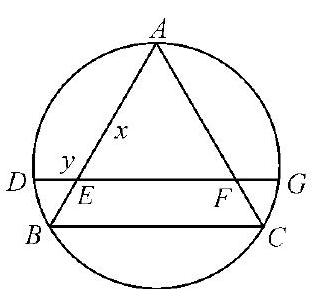
\includegraphics[max width=\textwidth, center]{2024_10_09_7e48ff928cc374c97394g-076}\\
	(第26题)

	中出现. $\square$\\
	28 求所有边长为整数且周长等于面积的两倍 (数值上) 的直角三角形的三边长.\\
	29 求边长为整数且面积等于 24 的直角三角形的三边长.\\
	30 已知 $\triangle A B C$ 的三边长都是整数, $\angle A=2 \angle B, \angle C>90^{\circ}$. 求 $\triangle A B C$ 的周长的最小值.\\
	31 设整数 $a ,  b$ 满足 $5 a \geqslant 7 b \geqslant 0$. 证明: 关于 $x ,  y ,  z, w$ 的方程组
\begin{align*}
		\left\{\begin{array}{l}
			       x+2 y+3 z+7 w=a \\
			       y+2 z+5 w=b
		       \end{array}\right.
	\end{align*}

	有非负整数解.\\
	32 正整数 $a ,  b ,  c$ 两两互素. 证明: 数 $2 a b c-a b-b c-c a$ 是不能表示为 $x b c+y c a+z a b$ 形式的最大正整数, 这里 $x ,  y ,  z$ 是非负整数.\\
	33 设 $n$ 为正整数, 用 $d(n)$ 表示 $n$ 的正因数的个数, $\varphi(n)$ 表示 $1,2, \cdots, n$ 中与 $n$ 互素的数的个数. 求所有的 $n$, 使得 $d(n)+\varphi(n)=n$.\\
	34 证明: 存在无穷多个三元正整数数组 $(a, b, c)$, 使得 $a^{2}+b^{2}, b^{2}+c^{2}, c^{2}+$ $a^{2}$ 都是完全平方数.\\
	35 证明: 不定方程 $x^{2}=y^{5}-4$ 没有整数解. \\
	36 证明: 不存在正整数 $m ,  n$, 使得 $19^{19}=m^{3}+n^{4}$.\\
	37 是否存在正整数 $x ,  y ,  z ,  u ,  v$, 使得 $x ,  y ,  z ,  u ,  v$ 都大于 2012, 且满足 $x^{2}+y^{2}+z^{2}+u^{2}+v^{2}=x y z u v-65$.\\
	38 求所有的整数 $a$, 使得方程 $x^{2}+a x y+y^{2}=1$, 有无穷多组整数解.\\
	39 求所有的正整数 $x ,  k ,  n(n \geqslant 2)$, 使得
\begin{align*}
		3^{k}-1=x^{n}
	\end{align*}

	40 求使得不定方程
\begin{align*}
		n=x^{3}-x^{2} y+y^{2}+x-y
	\end{align*}

	没有正整数解的最小正整数 $n$.

	

\section{习 题 2}
\begin{enumerate}
	\item 若 $p ,  q$ 都是奇数,则 $7 p+q$ 为偶数, 它不是素数, 故 $p ,  q$ 中有一个为偶数.
\end{enumerate}

情形一 设 $p$ 为偶数, 则 $p=2$ , 此时由 $7 p+q$ 为素数, 知 $q$ 为奇素数, 若 $q \neq 3$ , 则 $q \equiv 1$ 或 $2(\bmod 3)$ .

若 $q \equiv 1(\bmod 3) , $ 则
\begin{align*}
	7 p+q=14+q \equiv 0(\bmod 3)
\end{align*}

矛盾;

若 $q \equiv 2(\bmod 3) , $ 则
\begin{align*}
	p q+11=2 q+11 \equiv 4+11 \equiv 0(\bmod 3)
\end{align*}

亦矛盾, 所以 $q=3$, 此时
\begin{align*}
	7 p+q=17, p q+11=17
\end{align*}

都是素数,故
\begin{align*}
	\left(p^{2}+q^{p}\right)\left(q^{2}+p^{q}\right)=\left(2^{2}+3^{2}\right)\left(3^{2}+2^{3}\right)=221
\end{align*}

情形二 设 $q$ 为偶数, 则 $q=2$ . 同上讨论可知 $p=3$ , 此时
\begin{align*}
	\left(p^{2}+q^{p}\right)\left(q^{2}+p^{q}\right)=\left(3^{2}+2^{3}\right)\left(2^{2}+3^{2}\right)=221
\end{align*}

综上可知, 所求的值为 221 .\\
2. 设 $d$ 为公差, 则 $p_{1}, p_{1}+d, p_{1}+2 d, p_{1}+3 d, p_{1}+4 d$ 都是素数.

若 $2 \nmid d$ , 即 $d$ 为奇数, 则 $p_{1}+d$ 与 $p_{1}+2 d$ 中有一个为偶数, 它不是素数. \\
若 $3 \nmid d$ , 则 $p_{1}+d ,  p_{1}+2 d ,  p_{1}+3 d$ 中有一个为 3 的倍数(它们构成模 3 的一个完系), 矛盾.

若 $5 \nmid d$ , 则 $p_{1}, p_{1}+d, \cdots, p_{1}+4 d$ 中有一个是 5 的倍数, 只能是 $p_{1}=$ 5 , 这时公差 $d$ 是 6 的倍数.

而 $5,11,17,23,29$ 是 5 个成等差的素数数列, 所以,  $p_{5}$ 最小为 29 . \\
3. 注意到, 对任意正整数 $k, S(1 \underbrace{0 \cdots 08}_{k \uparrow})=9$ , 于是, 设 $1 \underbrace{0 \cdots 08}_{k \uparrow}=3 n$ , 则
\begin{align*}
	n=\underbrace{3 \cdots 36}_{k \uparrow},
\end{align*}

故 $S(n)=3 k+6$. 这样, 对任意正整数 $m$ , 取 $k=3 m-2$ , 就有
\begin{align*}
	S(n)=m S(3 n)
\end{align*}

说明 由 $S(3 n) \equiv 3 n(\bmod 9)$ , 故要求 $3 \mid S(n)$ , 进而 $3 \mid n$ , 所以在先确定 $3 n$ 时, 要寻找一个 9 的倍数(例如 $1 \underbrace{0 \cdots 02}_{k \uparrow}$ 作为 $3 n$ 就不能满足条件).

另外, 在 $S(2 n)$ 与 $S(n)$ 之间没有上述性质, 事实上, 可证:  $S(2 n) \leqslant$ $2 S(n) ;  S(n) \leqslant 5 S(2 n)$ . \\
4. 注意到, 当 $n$ 为偶数时, 设 $n=2 m$ , 有
\begin{align*}
	3^{n}=9^{m} \equiv 1(\bmod 8)
\end{align*}

当 $n=2 m+1$ 时, 
\begin{align*}
	3^{n}=9^{m} \times 3 \equiv 3(\bmod 8)
\end{align*}

所以, 对任意正整数 $n$ , 有
\begin{align*}
	3^{n}+1 \equiv 2 \text { 或 } 4(\bmod 8),
\end{align*}

故 $k \leqslant 2$. 又 $2^{2} \mid 3^{1}+1$ , 所以, 所求 $k$ 的最大值为 2 .

\section{5. 考虑数列}

\begin{align*}
	1,11,111, \cdots, \underbrace{1 \cdots 1}_{n+1 \uparrow},
\end{align*}

其中必有两个数对模 $n$ 同余 (因为任何整数除以 $n$ 所得的余数只能为 0,1 , $2 ,  \cdots ,  n-1$ , 共 $n$ 种情况), 它们的差(大的减小的)就是符合要求的 $m$ . \\
6. 如果 $(5, n)=1$, 那么由上题的结论, 知存在 $m=\underbrace{1 \cdots 1} \underbrace{0 \cdots 0}$, 使得 $n \mid m$ , 而 $n$ 为奇数, 结合 $5 \nmid n$ , 知 $(n, 10)=1$ , 故 $n \mid \underbrace{1 \cdots 1}$ . 命题获证.

如果 $5 \mid n$ , 设 $5^{\alpha} \| n$ , 那么可写 $n=5^{\alpha} \cdot n_{1}$ , 其中 $5 \nmid n_{1}$ . 利用 2.2 节例 5的结论, 可知存在一个 $\alpha$ 位的正整数 $m_{1}$ , 使得 $5^{\alpha} \mid m_{1}$ , 且 $m_{1}$ 的每个数码都是奇数, 这时, 考虑数
\begin{align*}
	m_{1}, \overline{m_{1} m_{1}}, \cdots, \overline{\underbrace{m_{1} \cdots m_{1}}_{n_{1}+1 \uparrow}}, \overline{i n c}
\end{align*}

这里 $\underbrace{\overline{m_{1} \cdots m_{1}}}$ 表示 $i$ 个 $m_{1}$ 连写形成的十进制数(故上面所列的数都是 $5^{\alpha}$ 的倍数), 则存在 $1 \leqslant i<j \leqslant n_{1}+1$, 使得
\begin{align*}
	\underbrace{\overline{m_{1} \cdots m_{1}}}_{j \uparrow} \equiv \underbrace{\overline{m_{1} \cdots m_{1}}}_{i \uparrow}\left(\bmod n_{1}\right)
\end{align*}

结合 $\left(n_{1}, 10\right)=1$ , 可知
\begin{align*}
	n_{1} \mid \underbrace{\overline{m_{1} \cdots m_{1}}}_{j-i \uparrow},
\end{align*}

于是记 $m=\underbrace{\overline{m_{1} \cdots m_{1}}}_{j-i \uparrow}$, 则 $m$ 中的每个数码都是奇数, 且

而
\begin{align*}
	5^{\alpha}\left|m, n_{1}\right| m
\end{align*}

故 $5^{\alpha} \cdot n_{1} \mid m$ , 即 $n \mid m$ . \\
命题获证. \\
7. 若 $n$ 为偶数,则
\begin{align*}
	19 \times 8^{n}+17 \equiv 1 \times(-1)^{n}+2 \equiv 0(\bmod 3) ;
\end{align*}

若 $n \equiv 1(\bmod 4)$ , 写 $n=4 k+1$ , 则\begin{align}
	19 \times 8^{n}+17 & =19 \times 64^{2 k} \times 8+17      \\
	                   & \equiv 6 \times(-1)^{2 k} \times 8+4 \\
	                   & \equiv 0(\bmod 13)
\end{align}

若 $n \equiv 3(\bmod 4) , $ 则\begin{align}
	19 \times 8^{n}+17 & =19 \times 64^{2 k+1} \times 8+17        \\
	                   & \equiv(-1) \times(-1)^{2 k+1} \times 3+2 \\
	                   & \equiv 0(\bmod 5)
\end{align}

所以, 对任意正整数 $n$ , 数 $19 \times 8^{n}+17$ 是合数.\\
8. 考虑数列 $\left\{F_{n}\right\}$ 中每一项除以 11(或 12)所得的余数. \\
(1) $\left\{F_{n}(\bmod 11)\right\}: 1,1,2,3,5,-3,2,-1,1,0,1,1, \cdots$ , 所以 $\left\{F_{n}(\bmod 11)\right\}$ 是以 10 为周期的纯周期数列, 因此\begin{align}
	       & \left\{F_{n}\right\} \text { 中任意连续 } 10 \text { 项之和 } \\
	\equiv & 1+1+2+3+5+(-3)+2+(-1)+1+0                                     \\
	=      & 11 \equiv 0(\bmod 11)
\end{align}

命题获证.\\
(2) $\left\{F_{n}(\bmod 12)\right\}: 1 ,  1 ,  3 ,  5 , -4 ,  1 , -3 , -2 , -5 ,  5 ,  0 ,  1 , $ $1 ,  \cdots$ 是以 12 为周期的纯周期数列. 直接验证, 可求出满足条件的最小正整数 $k=36$ .

说明 若 $k$ 是满足(2)的最小正整数, 而 $n$ 是满足(2)的正整数, 则 $k \mid n$ (这个结论请读者证明). 因此, 找到满足条件的 $n=36\left(\left\{F_{n}(\bmod 12)\right\}\right.$ 的每个周期内各数之和 $\equiv 4(\bmod 12))$ 后, 只需验证 36 的正因数不合要求, 就能断言 36 是符合条件的最小正整数.

\section{9. 先分别证明:}
 (1)若 $a^{2}+b^{2} \equiv 0(\bmod 3)$ , 则 $a \equiv b \equiv 0(\bmod 3)$ ; \\
(2)若 $a^{2}+b^{2} \equiv 0(\bmod 7)$ , 则 $a \equiv b \equiv 0(\bmod 7)$ . \\
这只需注意到, 对任意整数 $x$ , 都有
\begin{align*}
	x^{2} \equiv 0 \text { 或 } 1(\bmod 3),
\end{align*}

及
\begin{align*}
	x^{2} \equiv 0,1,2 \text { 或 } 4(\bmod 7),
\end{align*}

即可证出.

现在由 $21 \mid a^{2}+b^{2}$ 可推出 $21|a, 21| b$ , 故 $21^{2} \mid a^{2}+b^{2}$ , 所以命题成立.\\
10. 我们分别证明:\\
(1)若 $2 \mid c$ , 则 $2|a, 2| b$ ; \\
(2)若 $3 \mid c$ , 则 $3|a, 3| b$ ; \\
(3)若 $5 \mid c$ , 则 $5|a, 5| b$ . \\
(1) 的证明是平凡的. \\
(2)的证明只需注意到
\begin{align*}
	c^{2}=a^{2}+a b+b^{2}=(a-b)^{2}+3 a b
\end{align*}

就容易证出. \\
对于(3), 由条件, 知
\begin{align*}
	4 c^{2}=4 a^{2}+4 a b+4 b^{2}=3 a^{2}+(a+2 b)^{2}
\end{align*}

而对任意整数 $x$, 知
\begin{align*}
	x^{2} \equiv 0,1,4(\bmod 5)
\end{align*}

于是, 由
\begin{align*}
	3 x^{2}+y^{2} \equiv 0(\bmod 5)
\end{align*}

可知
\begin{align*}
	x^{2} \equiv y^{2} \equiv 0(\bmod 5)
\end{align*}

即
\begin{align*}
	x \equiv y \equiv 0(\bmod 5)
\end{align*}

因此,由 $5 \mid c$, 知

故
\begin{align*}
	\begin{gathered}
		3 a^{2}+(a+2 b)^{2} \equiv 0(\bmod 5) \\
		a \equiv a+2 b \equiv 0(\bmod 5)
	\end{gathered}
\end{align*}

可得
\begin{align*}
	a \equiv b \equiv 0(\bmod 5)
\end{align*}

所以(3)成立. \\
回到原题, 当 $c$ 是 2, 3 或 5 的倍数时,  $c^{2}=a^{2}+a b+b^{2}$ 两边可分别约去 $2^{2} ,  3^{2}$ 或 $5^{2}$ 后, 等式的形式保持不变. 所以 $c$ 有一个大于 5 的素因子. \\
11. (1)设表格中第 $i$ 行, 第 $j$ 列的方格上所填的数为 $a_{i j}, 1 \leqslant i \leqslant 3,1 \leqslant$ $j \leqslant 3$ , 则\begin{align}
	       & a_{11}+a_{22}+a_{33} \\
	\equiv & a_{13}+a_{22}+a_{31} \\
	\equiv & a_{12}+a_{22}+a_{32} \\
	\equiv & a_{21}+a_{22}+a_{23} \\
	\equiv & 0(\bmod 9),
\end{align}

于是, 它们求和后, 得
\begin{align*}
	\left(a_{11}+a_{12}+a_{13}+a_{21}+a_{22}+a_{23}+a_{31}+a_{32}+a_{33}\right)+3 a_{22} \equiv 0(\bmod 9)
\end{align*}

即
\begin{align*}
	3 a_{22}+(1+2+\cdots+9) \equiv 0(\bmod 9)
\end{align*}

故 $9 \mid 3 a_{22}$,

即
\begin{align*}
	3 \mid a_{22}
\end{align*}

从而表格中正当中的格子内所填数为 3 的倍数.\\
(2)下表给出的例子是中间格为 6 的一种填法.

\begin{center}
	\begin{tabular}{|l|l|l|}
		\hline
		9 & 5 & 4 \\
		\hline
		1 & 6 & 2 \\
		\hline
		8 & 7 & 3 \\
		\hline
	\end{tabular}
\end{center}

\begin{enumerate}
	\setcounter{enumi}{11}
	\item 一般地, 设数 $\overline{a_{n} a_{n-1} \cdots a_{0}}$ 是一个十进制表示下的 $n+1$ 位数,则若它是19的倍数, 那么
\begin{align*}
		      10 \overline{a_{n} a_{n-1} \cdots a_{1}}+a_{0}=\overline{a_{n} a_{n-1} \cdots a_{0}} \equiv 0(\bmod 19)
	      \end{align*}
\end{enumerate}

故
\begin{align*}
	20 \overline{a_{n} a_{n-1} \cdots a_{1}}+2 a_{0} \equiv 0(\bmod 19)
\end{align*}

即
\begin{align*}
	\overline{a_{n} a_{n-1} \cdots a_{1}}+2 a_{0} \equiv 0(\bmod 19)
\end{align*}

这表明每次操作后的结果都是 19 的倍数. \\
另一方面, 若
\begin{align*}
	\overline{a_{n} a_{n-1} \cdots a_{1}}+2 a_{0} \equiv 0(\bmod 19)
\end{align*}

则
\begin{align*}
	10 \overline{a_{n} a_{n-1} \cdots a_{1}}+20 a_{0} \equiv 0(\bmod 19)
\end{align*}

这表明
\begin{align*}
	10 \overline{a_{n} a_{n-1} \cdots a_{1}}+a_{0} \equiv 0(\bmod 19)
\end{align*}

即
\begin{align*}
	\overline{a_{n} a_{n-1} \cdots a_{0}} \equiv 0(\bmod 19)
\end{align*}

所以, 若某次操作后的结果是 19 的倍数, 则操作前该数也是 19 的倍数. \\
所以, 题给的判别方法是正确的. \\
对于 29 而言, 类似的判别方法是: 每次去掉最后一位, 将它的 3 倍与剩下的数相加, 依此类推, 直到变为 30 以内的数为止. 若最后的结果为 29 , 则原数是 29 的倍数, 否则原数不是 29 的倍数.

\section{3. 不能做到.}
事实上, 若存在满足条件的染色方式, 我们在黑格中都写上 +1 , 白格中都写上 -1 . 并依表格的中心所在的两条方格线将表格分为 4 块, 左上角那块中各数之和设为 $A$ , 右上角那块为 $B$ , 左下角那块为 $C$ , 右下角那块为 $D$ . 由条件, 可知 $A ,  B ,  C ,  D$ 都是 $1005^{2}$ 个奇数之和, 故 $A ,  B ,  C ,  D$ 都为奇数, 且 $A=-D, B=-C$ (因为关于表格的中心对称的方格不同色), 而且 $A+B=$ $A+C=0$ (这里用到每行, 每列中黑, 白格数各占一半). 所以 $A-C=A+$ $C=0$ , 这要求 $A=C=0$ , 但 $A ,  C$ 都是奇数, 矛盾.\\
14. 至少需要 3 次提问.

先证"3 次提问是足够的". 例如: \\
第一次为: $a_{1}, a_{2}, \cdots, a_{15}$ ; \\
第二次为: $a_{1}, a_{2}, \cdots, a_{8}, a_{16}, a_{17}, \cdots, a_{22}$ ; \\
第三次为: $a_{1}, a_{9}, a_{10}, \cdots, a_{22}$ . \\
其中 $a_{i}$ 表示第 $i$ 盒中火柴的数目. 这样,  3 个答案之和的奇偶性与 $a_{1}$ 的奇偶性相同(其余每盒在 3 次提问中各恰好出现 2 次). 因此, 经 3 次提问可确定 $a_{1}$ 的奇偶性.

再证"至少需要 3 次提问". 如果提问只有两次, 且两次中都出现 $a_{1}$ , 那么在两次提问中必有 $a_{i}$ 和 $a_{j}$ , 使得 $a_{i}$ 只在第 1 次提问中出现, 而 $a_{j}$ 只在第二次提问中出现, 这样同时改变 $a_{1} ,  a_{i} ,  a_{j}$ 的奇偶性, 每次答案是相同的, 从而不能确定 $a_{1}$ 的奇偶性. 如果两次中不都出现 $a_{1}$, 在 $a_{1}$ 都不出现时, 改变 $a_{1}$ 的奇偶性; 在 $a_{1}$ 只出现一次时, 改变 $a_{1}$ 与 $a_{i}$ (这里 $a_{i}$ 是与 $a_{1}$ 同时出现的某个火柴盒)的奇偶性, 那么两次答案仍是相同的, 不能确定 $a_{1}$ 的奇偶性.

综上可知, 至少需要提问 3 次. \\
15. 用 $a_{i j}$ 表示第 $i$ 行, 第 $j$ 列上的方格内所填的数. 如果存在符合要求的填法, 那么我们不妨设 $a_{11}=1$ (否则改变表格中所有数的符号再讨论), 此时 $a_{21}$ 与 $a_{12}$ 中恰有一个为 -1 , 不妨设 $a_{21}=-1$ (否则将表格的第 2 行与第 2 列互换后再讨论), 则 $a_{12}=1$ , 进一步讨论, 知 $a_{22}=-1, a_{13}=1, \cdots$ , 可知第 1行中的数都是1, 第2行中的数都是 -1 , 进而, 第 3 行中的数都是 -1 , 第 4 行中的数都是 1 , 依此递推, 知当且仅当 $i \equiv 1(\bmod 3)$ 时, 第 $i$ 行中的数都是 1 , 而其余每行中的数都是 -1 . 如果 $n \equiv 0(\bmod 3)$ , 那么第 $n$ 行的数为 -1 , 该行上的每个方格中相邻方格上的数都是 -1 , 不合要求, 直接验证可知其余情况都合要求.

所以, 当且仅当 $3 \nmid n, n>1$ 时,存在符合要求的填法.\\
16. 若 $r_{1}, r_{2}, \cdots, r_{100}$ 中只有 10 个不同的数,则对 $i=1,2, \cdots, 99$,\\
$r_{i+1}-r_{i}$ 只有 $10^{2}-9=91$ (这里减去 9 是因为 $r_{i+1}=r_{i}$ 时所得的值都是零)种不同取值. 但是在模 100 的意义下,  $r_{i+1}-r_{i}$ 依次为 $a_{2}, a_{3}, \cdots, a_{100}$ , 共有 99种不同的取值, 矛盾.

所以,  $r_{1}, r_{2}, \cdots, r_{100}$ 中至少有 11 个不同的值.\\
17. 若 $a$ 是一个满足条件的数,则 $a^{x_{0}}>1$, 故 $a>1$. 此时, 对
\begin{align*}
	a^{x_{0}}=a^{x_{1}}+a^{x_{2}}+\cdots+a^{x_{2001}}
\end{align*}

两边模 $a-1$ , 知 $\quad 1 \equiv \underbrace{1+\cdots+1}_{2001 \uparrow}(\bmod a-1) , $\\
所以
\begin{align*}
	a-1 \mid 2000
\end{align*}

另一方面, 若 $a>1$ , 满足 $a-1 \mid 2000$ , 则我们在 $x_{1}, x_{2}, \cdots, x_{2001}$ 中取 $a$个数为 $0, a-1$ 个为 $1, a-1$ 个为 $2, \cdots, a-1$ 个为 $k-1$, 这里 $k=\frac{2000}{a-1}$,并取 $x_{0}=k$ , 就有 $a^{x_{0}}=a^{x_{1}}+a^{x_{2}}+\cdots+a^{x_{2001}}$ .

所以, 当且仅当 $a>1$ 且 $a-1 \mid 2000$ 时, $a$ 为满足条件的数, 这样的 $a$ 共有 20 个.\\
18. 若 $m\left(2^{m}-1\right) \mid n$, 设 $n=m\left(2^{m}-1\right) k$, 则\begin{align}
	2^{n}-1 & =2^{m\left(2^{m}-1\right) k}-1                 \\
	        & =\left(2^{m k}\right)^{\left(2^{m}-1\right)}-1 \\
	        & =\left(2^{m k}-1\right) A
\end{align}

其中
\begin{align*}
	A=\left(2^{m k}\right)^{2^{m}-2}+\left(2^{m k}\right)^{2^{m}-3}+\cdots+\left(2^{m k}\right)^{1}+1
\end{align*}

注意到
\begin{align*}
	\begin{gathered}
		2^{m k}-1=\left(2^{m}\right)^{k}-1 \equiv 1^{k}-1 \equiv 0\left(\bmod 2^{m}-1\right) \\
		A \equiv 1^{2^{m}-2}+1^{2^{m}-3}+\cdots+1^{1}+1=2^{m}-1 \equiv 0\left(\bmod 2^{m}-1\right)
	\end{gathered}
\end{align*}

所以
\begin{align*}
	\left(2^{m}-1\right)^{2} \mid 2^{n}-1
\end{align*}

反过来, 若 $\left(2^{m}-1\right)^{2} \mid 2^{n}-1$ , 我们先证 $m \mid n$ . 若否, 设 $n=m q+r, 0<$ $r<m$ , 则由
\begin{align*}
	2^{n} \equiv 1\left(\bmod 2^{m}-1\right)
\end{align*}

知
\begin{align*}
	\left(2^{m}\right)^{q} \cdot 2^{r} \equiv 1\left(\bmod 2^{m}-1\right)
\end{align*}

故
\begin{align*}
	2^{r} \equiv 1\left(\bmod 2^{m}-1\right)
\end{align*}

但是
\begin{align*}
	1 \leqslant 2^{r}-1<2^{m}-1
\end{align*}

所以 $2^{m}-1 \nmid 2^{r}-1$ , 矛盾. 因此 $m \mid n$.\\
现设 $n=m q$ , 则
\begin{align*}
	2^{n}-1=\left(2^{m}-1\right) \times B
\end{align*}

其中
\begin{align*}
	B=\left(2^{m}\right)^{q-1}+\left(2^{m}\right)^{q-2}+\cdots+2^{m}+1
\end{align*}

由
\begin{align*}
	\left(2^{m}-1\right)^{2} \mid 2^{n}-1
\end{align*}

知
\begin{align*}
	2^{m}-1 \mid B
\end{align*}

又
\begin{align*}
	B \equiv 1^{q-1}+1^{q^{-2}}+\cdots+1=q\left(\bmod 2^{m}-1\right)
\end{align*}

所以
\begin{align*}
	2^{m}-1 \mid q
\end{align*}

从而
\begin{align*}
	m\left(2^{m}-1\right) \mid n
\end{align*}

命题获证.\\
19. 记 $A=\frac{a^{p}+b^{p}}{a+b}=a^{p-1}-a^{p-2} b+\cdots-a b^{p-2}+b^{p-1}$ , 结合 $p$ 为奇数及 $b \equiv-a(\bmod a+b)$ , 知
\begin{align*}
	A \equiv \underbrace{a^{p-1}+a^{p-1}+\cdots+a^{p-1}}_{p \uparrow}=p a^{p-1}(\bmod a+b) .
\end{align*}

而
\begin{align*}
	(a, b)=1
\end{align*}

故
\begin{align*}
	(a, a+b)=1
\end{align*}

所以\begin{align}
	\left(a+b, \frac{a^{p}+b^{p}}{a+b}\right) & =(a+b, A)                    \\
	                                          & =\left(a+b, p a^{p-1}\right) \\
	                                          & =(a+b, p)=1 \text { 或 } p .
\end{align}\\
20. 由条件, 知 $65 \mid(18+9 a)$ (取 $x=1$ ), 而 $(9,65)=1$, 故 $65 \mid a+2$,即 $a \geqslant 63$.

当 $a=63$ 时,利用 Fermat 小定理知: 对任意整数 $x$ , 都有\begin{align}
	       & 5 x^{13}+13 x^{5}+9 a x \\
	\equiv & 13 x+9 a x              \\
	\equiv & (3+(-1) \times 3) x     \\
	\equiv & 0(\bmod 5)              \\
	       & 5 x^{13}+13 x^{5}+9 a x
\end{align}\begin{align}
	 & \equiv 5 x+9 a x         \\
	 & \equiv(5+9 \times(-2)) x \\
	 & \equiv 0(\bmod 13)
\end{align}

所以
\begin{align*}
	65 \mid 5 x^{13}+13 x^{5}+9 a x
\end{align*}

综上可知, 所求的最小正整数 $a=63$.\\
21. 不存在这样的整数 $a ,  b ,  c$ .

事实上, 若 $a ,  b ,  c$ 满足条件, 我们不妨设 $a$ 为偶数(否则用 $-(a+1)$ ,  $-(b+1) , -(c+1)$ 代替 $a ,  b ,  c$ 讨论), 由条件, 结合韦达定理知 $-\frac{b}{a}$ 与 $\frac{c}{a}$ 都是整数, 故 $b ,  c$ 都是偶数, 所以 $a+1 ,  b+1 ,  c+1$ 都是奇数. 此时, 对任意整数 $x$ , 有\begin{align}
	       & (a+1) x^{2}+(b+1) x+(c+1) \\
	\equiv & x^{2}+x+1                 \\
	=      & x(x+1)+1                  \\
	\equiv & 1(\bmod 2)
\end{align}\\
(最后一步用到 $x$ 与 $x+1$ 中有一个偶数). 这表明方程 $(a+1) x^{2}+(b+1) x+$ $(c+1)=0$ 没有整数根, 矛盾. \\
22. 不妨设 $x \leqslant y \leqslant z<w$, 则 $w \geqslant z+1$, 若 $z \geqslant 3$, 则
\begin{align*}
	w!\geqslant(z+1) \cdot(z!) \geqslant 4 \cdot(z!)>z!+y!+x!
\end{align*}

矛盾, 故
\begin{align*}
	z \leqslant 2
\end{align*}

若 $z=1$ , 则 $x=y=z=1$ , 此时 $w!=3$ , 不存在这样的 $w$ , 故 $z=2$ . 此时 $w \geqslant 3$ , 故
\begin{align*}
	w!\equiv 0(\bmod 3)
\end{align*}

所以
\begin{align*}
	x!+y!\equiv 1(\bmod 3)
\end{align*}

而
\begin{align*}
	x \leqslant y \leqslant 2
\end{align*}

故只能是
\begin{align*}
	x=y=2
\end{align*}

此时
\begin{align*}
	w=3,
\end{align*}

故
\begin{align*}
	(x, y, z, w)=(2,2,2,3)
\end{align*}\\
23. 注意到, $a^{2}+b^{2} \equiv a^{2}-36 b^{2}(\bmod 37)$ , 故由条件知
\begin{align*}
	37 \mid a^{2}-36 b^{2}
\end{align*}

即
\begin{align*}
	37 \mid(a-6 b)(a+6 b)
\end{align*}

所以\\
$37 \mid a-6 b$ 或 $37 \mid a+6 b$.\\
因此, 对每个 $1 \leqslant b \leqslant 36$ , 可知恰有两个 $a(a \equiv \pm 6 b(\bmod 37))$ 满足条件, 而 $b=0$ 时, 由 $a^{2}+b^{2} \equiv 0(\bmod 37)$ 知 $a=0$ . 所以, 满足条件的 $(a, b)$ 共有 $2 \times 36+1=73$ (组). \\
24. 由条件可设 $m^{2}+n^{2}+m=k m n, k$ 为正整数, 这样, 关于 $n$ 的一元二次方程
\begin{align*}
	n^{2}-k m n+m^{2}+m=0
\end{align*}

有正整数解, 故
\begin{align*}
	\Delta=(k m)^{2}-4\left(m^{2}+m\right)=m\left(k^{2} m-4 m-4\right)
\end{align*}

\section{是一个完全平方数. }
若 $m$ 为奇数, 则
\begin{align*}
	\left(m, k^{2} m-4 m-4\right)=(m,-4)=1
\end{align*}

故由 $\Delta$ 为完全平方数知 $m$ 为完全平方数. \\
若 $m$ 为偶数, 则由 (1)知 $n$ 为偶数(否则(1)的左边为奇数, 矛盾), 故 $4 \mid n^{2}$ ,  $4|k m n ,  4| m^{2}$ , 从而由(1)知 $4 \mid m$ . 设 $m=4 m_{1}$ , 则
\begin{align*}
	\Delta=16 m_{1}\left(k^{2} m_{1}-m_{1}-1\right)
\end{align*}

所以, $m_{1}\left(k^{2} m_{1}-m_{1}-1\right)$ 是一个完全平方数, 这时
\begin{align*}
	\left(m_{1}, k^{2} m_{1}-m_{1}-1\right)=\left(m_{1},-1\right)=1
\end{align*}

故 $m_{1}$ 是完全平方数. 所以 $m=4 m_{1}$ 也是完全平方数. 命题获证.\\
25. 设 $n=x^{2}+y^{2}+z^{2}, x \geqslant y \geqslant z$ 为正整数,则\begin{align}
	n^{2} & =\left(x^{2}+y^{2}+z^{2}\right)^{2}                                 \\
	      & =\left(x^{2}+y^{2}\right)^{2}+2\left(x^{2}+y^{2}\right) z^{2}+z^{4} \\
	      & =\left(x^{2}+y^{2}-z^{2}\right)^{2}+4\left(x^{2}+y^{2}\right) z^{2} \\
	      & =\left(x^{2}+y^{2}-z^{2}\right)^{2}+(2 x z)^{2}+(2 y z)^{2} .
\end{align}

注意到,  $x^{2}+y^{2}-z^{2}>0$ , 知 $n^{2}$ 可表为 3 个正整数的平方和. \\
26. 设 $n=1000 x+y$, 这里 $x$ 为正整数, $y$ 为整数,且 $0 \leqslant y \leqslant 999$ . 依题意知
\begin{align*}
	x^{3}=1000 x+y
\end{align*}

由 $0 \leqslant y \leqslant 999$ , 知

故
\begin{align*}
	1000 x \leqslant x^{3}<1000 x+1000=1000(x+1)
\end{align*}

得
\begin{align*}
	x^{2} \geqslant 1000, x^{3}+1 \leqslant 1000(x+1)
\end{align*}

所以
\begin{align*}
	x^{2} \geqslant 1000, x^{2}-x+1 \leqslant 1000
\end{align*}

故
\begin{align*}
	32 \leqslant x<33
\end{align*}
\begin{align*}
	x=32
\end{align*}

这样
\begin{align*}
	y=768
\end{align*}

所以
\begin{align*}
	n=32768
\end{align*}\\
27. 只需寻找正整数 $l$, 使得 $l^{2}-1=x^{2}+y^{2}$ 有正整数解. 令 $x=2 m^{2}$, $y=2 m$ , 及 $l=2 m^{2}+1$ , 就有 $l^{2}-1=x^{2}+y^{2}$ . 所以, 对任意正整数 $m$ , 取

则
\begin{align*}
	n=\left(2 m^{2}+1\right)^{2}-1=4 m^{4}+4 m^{2}
\end{align*}\\
28. 由条件,知 $n^{3} \equiv 888(\bmod 1000)$ , 故
\begin{align*}
	n^{3} \equiv 888(\bmod 8), n^{3} \equiv 888(\bmod 125)
\end{align*}

由前者知 $n$ 为偶数, 设 $n=2 m$ , 则
\begin{align*}
	m^{3} \equiv 111(\bmod 125)
\end{align*}

因此
\begin{align*}
	m^{3} \equiv 111 \equiv 1(\bmod 5)
\end{align*}

注意到当 $m=0,1,2,3,4(\bmod 5)$ 时, 对应地
\begin{align*}
	m^{3} \equiv 0,1,3,2,4(\bmod 5)
\end{align*}

所以, 由 $m^{3} \equiv 1(\bmod 5)$ 知 $m \equiv 1(\bmod 5)$ , 可设 $m=5 k+1$ , 这时
\begin{align*}
	m^{3}=(5 k+1)^{3}=125 k^{3}+75 k^{2}+15 k+1 \equiv 111(\bmod 125)
\end{align*}

故
\begin{align*}
	75 k^{2}+15 k \equiv 110(\bmod 125)
\end{align*}

从而
\begin{align*}
	15 k^{2}+3 k \equiv 22(\bmod 25)
\end{align*}

即有
\begin{align*}
	15 k^{2}+3 k+3 \equiv 0(\bmod 25)
\end{align*}

故
\begin{align*}
	5 k^{2}+k+1 \equiv 0(\bmod 25)
\end{align*}

这要求
\begin{align*}
	5 k^{2}+k+1 \equiv 0(\bmod 5)
\end{align*}

故
\begin{align*}
	5 \mid k+1
\end{align*}

可设 $k+1=5 l$, 得\begin{align}
	 & 5 k^{2}+k+1=5 \times(5 l-1)^{2}+5 l \\
	 & =125 l^{2}-50 l+5(l+1)              \\
	 & \equiv 0(\bmod 25) \text { ,  }     \\
	 & 5 \mid l+1 \text {. }
\end{align}

故\\
可设 $l+1=5 r$ , 因此\begin{align}
	n & =2 m=10 k+2=10(5 l-1)+2 \\
	  & =50 l-8=50(5 r-1)-8     \\
	  & =250 r-58
\end{align}

结合 $n$ 为正整数, 可知
\begin{align*}
	n \geqslant 250-58=192
\end{align*}

又 $192^{3}=7077888$ 符合要求,故满足条件的最小正整数为 192 .\\
29. 由于 $n \geqslant 2$, 故 $2^{n}-1 \equiv-1(\bmod 4)$, 而完全平方数 $\equiv 0$ 或 $1(\bmod 4)$,故 $2^{n}-1$ 不是完全平方数.

另一方面, 若存在 $n>1$ 及正整数 $x$, 使得

则
\begin{align*}
	\begin{gathered}
		2^{n}-1=x^{3} \\
		2^{n}=(x+1)\left(x^{2}-x+1\right) \\
		x^{2}-x+1=x(x-1)+1
	\end{gathered}
\end{align*}

由于\\
其中 $x(x-1)$ 为偶数 (两个相邻整数中有一个为偶数), 故 $x^{2}-x+1$ 为奇数,这要求
\begin{align*}
	x^{2}-x+1=1
\end{align*}

进而 $x=1$ , 导出 $n=1$ , 矛盾. 故 $2^{n}-1$ 不是一个完全立方数.\\
30. 先证: 对任意正整数 $a$, 若 $\sqrt{a}$ 为有理数, 则 $a$ 为完全平方数.

事实上, 若 $\sqrt{a}=\frac{q}{p}, p ,  q$ 为正整数, 且 $(p, q)=1$, 则 $a=\frac{q^{2}}{p^{2}}$, 此时由 $a$为正整数, 知 $p^{2} \mid q^{2}$, 但 $(p, q)=1$ , 故 $p=1$ , 即 $a=q^{2}$ .

再证原题: 设 $\sqrt{a}+\sqrt{b}+\sqrt{c}=m, m$ 为整数, 则
\begin{align*}
	(\sqrt{a}+\sqrt{b})^{2}=(m-\sqrt{c})^{2},
\end{align*}

即
\begin{align*}
	a+b+2 \sqrt{a b}=m^{2}-2 \sqrt{c}+c
\end{align*}

于是 $\sqrt{a b}+\sqrt{c}$ 为有理数. 进而可设 $\sqrt{a b}+\sqrt{c}=n, n$ 为正有理数, 则
\begin{align*}
	a b=(n-\sqrt{c})^{2}=n^{2}-2 n \sqrt{c}+c,
\end{align*}

故 $\sqrt{c}$ 为有理数. 利用前面的结论可知 $c$ 为完全平方数, 因此 $\sqrt{a}+\sqrt{b}=m-\sqrt{c}$为正整数. 同上处理可知 $a ,  b$ 也都是完全平方数. \\
31. 通过凑完全平方式来处理. 由条件可设 $c=p q, 3 \leqslant p \leqslant q, p ,  q$ 都是奇数, 现在需要寻找 $a$ , 使得 $(2 a-1)^{2}+8 p q$ 是一个完全平方式, 一个自然的取法是: 令 $2 a-1=2 q-p$ , 则\begin{align}
	(2 a-1)^{2}+8 p q & =(2 q-p)^{2}+8 p q \\
	                  & =(2 q+p)^{2}
\end{align}

这时\begin{align}
	a & =\frac{1}{2}(2 q-p+1)       \\
	  & =q-\frac{p-1}{2}            \\
	  & \leqslant q-1=\frac{c}{p}-1 \\
	  & \leqslant \frac{c}{3}-1
\end{align}

符合题中的要求.\\
32. 若 $a \neq 0$, 注意到在 $a<0$ 时, $n$ 充分大后, 数 $2^{n} a+b<0$, 与 $2^{n} a+b$为完全平方数矛盾, 故 $a>0$ . 现在设 $2^{n} a+b=x_{n}^{2}, x_{n}$ 为正整数, 则对任意正整数 $n$ , 有 $x_{n}<x_{n+1}$ .

由于 $4 x_{n}^{2}-x_{n+2}^{2}=4\left(2^{n} a+b\right)-\left(2^{n+2} a+b\right)=3 b$,\\
故
\begin{align*}
	3|b|=\left|2 x_{n}-x_{n+2}\right| \cdot\left|2 x_{n}+x_{n+2}\right|
\end{align*}

而 $2 x_{n}+x_{n+2}$ 随着 $n$ 的增大而增大, 故只能是
\begin{align*}
	\left|2 x_{n}-x_{n+2}\right|=0
\end{align*}

即
\begin{align*}
	|b|=0
\end{align*}

但这时 $2^{n} a$ 与 $2^{n+1} a$ 都要是完全平方数, 这是不可能的, 矛盾. 所以 $a=0$ . \\
33. 对任意不能表示为 42 的正倍数与一个合数之和的正整数 $n$, 考虑 $n$除以 42 所得的余数 $r$ . 若 $r=0$ 或 $r$ 为合数, 则 $n \leqslant 42$ .

下面考虑 $r=1$ 或 $r$ 为素数的情形. \\
若 $r \equiv 1(\bmod 5)$ , 则
\begin{align*}
	\begin{gathered}
		84+r \equiv 0(\bmod 5) \\
		n<3 \times 42=126
	\end{gathered}
\end{align*}

此时\\
若 $r \equiv 2(\bmod 5) , $ 则
\begin{align*}
	4 \times 42+r \equiv 0(\bmod 5)
\end{align*}

此时
\begin{align*}
	n<5 \times 42=210
\end{align*}

若 $r \equiv 3(\bmod 5) , $ 则

此时
\begin{align*}
	\begin{gathered}
		42+r \equiv 0(\bmod 5) \\
		n<2 \times 42=84
	\end{gathered}
\end{align*}

若 $r \equiv 4(\bmod 5)$ , 则
\begin{align*}
	3 \times 42+r \equiv 0(\bmod 5)
\end{align*}

此时
\begin{align*}
	n<4 \times 42=168
\end{align*}

若 $r \equiv 0(\bmod 5) , $ 则
\begin{align*}
	r=5
\end{align*}

此时由于 $5,47,89,131,173$ 都是素数,故 $n$ 最大为 215 . \\
综上可知, 所求最大正整数为 215 .\\
34. 由于 $30030=2 \times 3 \times 5 \times 7 \times 11 \times 13$ , 所以若取 $N=210 k$ , 则 $N$ 与 $N \pm r$ 都与 30030 不互素, 这里 $r$ 为 $2,3, \cdots, 10$ 中的数. 现在考虑数 $N \pm 1$ , 我们取 $k$ , 使得
\begin{align*}
	210 k \equiv 1(\bmod 11) \text { 且 } 210 k \equiv-1(\bmod 13),
\end{align*}

前者要求 $k \equiv 1(\bmod 11)$, 设 $k=11 m+1$,\\
后者要求
\begin{align*}
	210(11 m+1) \equiv-1(\bmod 13)
\end{align*}

解得
\begin{align*}
	m \equiv 4(\bmod 13)
\end{align*}

所以, 令 $k=45$ , 则所得的 21 个数 $9440,9441, \cdots, 9460$ 与 30030 都不互素, 因此取 $n=9440$ 即可. \\
35. 注意到,  $114,115, \cdots, 126$ 这 13 个数都是合数, 每个数都是 $2 ,  3$ ,  $5 ,  7 ,  11$ 中某个数的倍数, 因此存在 13 个符合要求的数.

下证: 没有连续 14 个正整数, 使得其中每个数都是 $2 ,  3 ,  5 ,  7 ,  11$ 中某个数的倍数.

事实上, 若存在这样的 14 个数, 考虑其中的 7 个奇数, 设它们为 $a ,  a+2, \cdots$ ,  $a+12$. 由于若两个奇数都是 3 的倍数, 则它们的差至少为 6 , 故这 7 个奇数中至多有 3 个数是 3 的倍数.

同样可证这 7 个奇数中至多有 2 个数是 5 的倍数; 至多有 1 个数为 7 的倍数; 至多有 1 个数为 11 的倍数.

由假设, 这 7 个数都是 $3 ,  5 ,  7 ,  11$ 中某个数的倍数, 故这 7 个奇数中分别有 3 个为 3 的倍数,  2 个为 5 的倍数,  1 个为 7 的倍数,  1 个为 11 的倍数, 并且不出现一个数同时是 $3 ,  5 ,  7 ,  11$ 中某两个数的倍数. 但是, 这时要求 $a$ ,  $a+6 ,  a+12$ 为 3 的倍数;  $a ,  a+10$ 或者 $a+2 ,  a+12$ 中有一组数为 5 的倍数. 必有一个数同为 3 和 5 的倍数, 矛盾. \\
36. 当 $p=2$ 时, $a^{n}=13$ , 知 $a=13, n=1$ . 当 $p>2$ 时,由 $p$ 为素数,可知 $p$ 为奇数, 此时
\begin{align*}
	2^{p}+3^{p}=(2+3)\left(2^{p-1}-2^{p-2} \times 3+\cdots-2 \times 3^{p-2}+3^{p-1}\right)
\end{align*}

故 $5 \mid a^{n}$ , 即 $5 \mid a$ . 若 $n>1$ , 则 $5^{2} \mid a^{n}$ , 这时, 应有
\begin{align*}
	2^{p-1}-2^{p-2} \times 3+\cdots-2 \times 3^{p-2}+3^{p-1} \equiv 0(\bmod 5)
\end{align*}

利用 $3 \equiv-2(\bmod 5), p$ 为奇数及上式, 知\begin{align}
	       & 2^{p-1}-2^{p-2} \times 3+\cdots-2 \times 3^{p-2}+3^{p-1}                      \\
	\equiv & \underbrace{\underbrace{p \uparrow 2^{p-1}}}_{2^{p-1}+2^{p-1}+\cdots+2^{p-1}} \\
	=      & p \cdot 2^{p-1} \equiv 0(\bmod 5),
\end{align}

所以,  $5 \mid p$ , 而 $p$ 为素数, 故 $p=5$ , 这导致 $a^{n}=2^{5}+3^{5}=275=5^{2} \times 11 ,  n$只能为 1 , 矛盾.

因此,  $n=1$ . \\
37. 等价于求最小的正整数 $n$,使得
\begin{align*}
	1+2+\cdots+n \equiv 1+2+\cdots+2000(\bmod 2000)
\end{align*}

即
\begin{align*}
	\frac{n(n+1)}{2} \equiv 1000(\bmod 2000)
\end{align*}

等价于
\begin{align*}
	n(n+1) \equiv 2000(\bmod 4000)
\end{align*}

这要求
\begin{align*}
	2000 \mid n(n+1)
\end{align*}

注意到
\begin{align*}
	(n, n+1)=1
\end{align*}

而
\begin{align*}
	2000=2^{4} \times 5^{3}
\end{align*}

所以 $2^{4}\left|n ,  5^{3}\right| n+1$ ; 或者 $5^{3}\left|n ,  2^{4}\right| n+1$ ; 或者 $n$ 与 $n+1$ 中有一个为 2000的倍数. 分别求得 $n$ 最小为 $624,1375,1999$, 其中满足(1)的最小的数为 624.

所以, 被标上 2000 的那个点上所标的数中最小的那个是 624 .\\
38. 等价于求在模 800 的意义下,数列 $a, 2 a, 2^{2} a, 2^{3} a, \cdots$ 中, 出现的不同的数的个数的最大值, 这里 $a$ 在 $1,2, \cdots, 800$ 中取值.

注意到, 当 $2^{n} \neq 2^{m}(\bmod 800)$ 时,  $2^{n} a \neq 2^{m} a(\bmod 800)$ 不一定成立; 反过来, 当 $2^{n} a \not 2^{m} a(\bmod 800)$ 成立时,  $2^{n} \neq 2^{m}(\bmod 800)$ 一定成立. 因此, 数列 $a, 2 a, 2^{2} a, \cdots$ 在模 800 的意义下, 不同元素个数的最大值在 $a=1$ 时可以取到, 因此, 只需求 $1,2,2^{2}, \cdots$ 在模 800 的意义下不同元素的个数.

由于 $800=2^{5} \times 5^{2}$ , 而 $n \geqslant 5$ 时有
\begin{align*}
	2^{n} \equiv 0\left(\bmod 2^{5}\right)
\end{align*}

另外 $\left\{2^{n}(\bmod 25)\right\}$ 为: $2,4,8,16,7,14,3,6,12,-1,-2,-4,-8$, $-16,-7,-14,-3,-6,-12,1, \cdots$ , 故 $\left\{2^{n}(\bmod 25)\right\}$ 中恰有 20 个不同元素. 结合 $\left\{2^{n}\left(\bmod 2^{5}\right)\right\}$ 为 $2,4,8,16,0,0, \cdots$ , 可得 $\left\{2^{n}(\bmod 800)\right\}$ 中共有 $20+4=24$ (个)不同的数.

所以, 圆周上至多有 24 个点染成了红色. \\
39. 如果能确定 $a+b$ 的值(视 $m$ 为常数), 那么利用韦达定理的逆定理, 可知至多只有一组正整数 $(a, b)$ 满足条件.

由条件, 知 $(a+b)^{2}=(a-b)^{2}+4 a b$ 满足\begin{align}
	1+4 m & \leqslant(a+b)^{2}     \\
	      & <5+4 \sqrt{4 m+1}+4 m  \\
	      & =(\sqrt{4 m+1}+2)^{2},
\end{align}

即
\begin{align*}
	\sqrt{4 m+1} \leqslant a+b<\sqrt{4 m+1}+2
\end{align*}

所以
\begin{align*}
	a+b=\left\{\begin{array}{l}
		           \sqrt{4 m+1} \text { 或 } \sqrt{4 m+1}+1, \text { 若 } \sqrt{4 m+1} \text { 为整数; } \\
		           {[\sqrt{4 m+1}]+1 \text { 或 }[\sqrt{4 m+1}]+2, \text { 若 } \sqrt{4 m+1} \text { 不是整数. }}
	           \end{array}\right.
\end{align*}

总之,  $a+b$ 只能取值于某两个连续正整数. 而 $a b=m \equiv 2(\bmod 4)$ , 可知 $a ,  b$ 一奇一偶, 即 $a+b$ 为奇数. 这样我们知道 $a+b$ 的值唯一确定, 命题获证. \\
40. 用反证法, 若 $n$ 的每个素因子都不大于 10 , 利用条件,知 $n$ 为奇数,且 $n$ 不是 5 的倍数, 故存在非负整数 $i ,  j$ , 使得
\begin{align*}
	n=3^{i} \cdot 7^{j}
\end{align*}

考虑 $3^{i}$ 与 $7^{j}$ 除以 20 所得的余数, 对 $i=0,1,2, \cdots, j=0,1,2, \cdots$,分别依次有\begin{align}
	 & \left\{3^{i}(\bmod 20)\right\}: 1,3,9,7,1,3, \cdots \\
	 & \left\{7^{j}(\bmod 20)\right\}: 1,7,9,3,1,7, \cdots
\end{align}

这两个都是以 4 为周期循环的数列, 因此
\begin{align*}
	3^{i} \cdot 7^{j} \equiv a b(\bmod 20)
\end{align*}

这里 $a ,  b$ 都为 $1,3,7$ 或 9 . 分别计算, 可知
\begin{align*}
	3^{i} \cdot 7^{j} \equiv 1,3,7 \text { 或 } 9(\bmod 20),
\end{align*}

这表明, 所有形如 $3^{i} \cdot 7^{j}$ 的数的十位数字都为偶数, 但 $n$ 的每一位数字都是 1 , 3,7 或 9 , 矛盾.

所以, $n$ 有一个大于 10 的素因子. \\
41. 由条件可知 $p \neq q$, 利用对称性, 不妨设 $p<q$.

若 $p=2$ , 则 $q^{q}+5 \equiv 0(\bmod q)$ , 知 $q=5$ . 直接验证, 可知 $(p, q)=(2,5)$符合要求.

若 $p>2$ , 则 $p ,  q$ 都为奇素数. 由条件知 $p^{p}+1 \equiv 0(\bmod q)$ , 故 $p^{2 p} \equiv$ $1(\bmod q)$ , 利用 Fermat 小定理, 有 $p^{q-1} \equiv 1(\bmod q)$ , 于是, 
\begin{align*}
	p^{(2 p, q-1)} \equiv 1(\bmod q)
\end{align*}

注意到, $2 \mid(2 p, q-1)$, 而 $(2 p, q-1) \mid 2 p$, 故只有下面的两种情形.\\
情形一 $(2 p, q-1)=2$ , 则由 (1) 知 $p^{2} \equiv 1(\bmod q)$ , 导致 $q \mid p+1$ 或 $q \mid p-1$,这与 $p \leqslant q-2$ 矛盾.

情形二 $(2 p, q-1)=2 p$ , 则 $q \equiv 1(\bmod p) , $ 于是
\begin{align*}
	0 \equiv p^{p}+q^{q}+1 \equiv 1^{q}+1=2(\bmod p)
\end{align*}

导致 $p=2$ , 矛盾.\\
综上可知, 满足条件的 $(p, q)=(2,5)$ 或 $(5,2)$.\\
42. 若存在 $2 \leqslant m \leqslant 2010$ , 使得对某个正整数 $n$ , 有 $m \mid f(n)$ . 则由于 $f(1)=2011$ 为素数 (这里 2011 为素数需要对不大于 $\sqrt{2011}$ 的素数逐个除 2011 去验证), 故 $n \neq 1$ , 此时可写 $f(n)=\frac{n^{2011}-1}{n-1}$ .

对 $m$ 的素因子 $p$, 由 $m \mid f(n)$ 知 $n^{2011} \equiv 1(\bmod p)$ , 而由 Fermat 小定理知 $n^{p-1} \equiv 1(\bmod p)$ , 所以, 有
\begin{align*}
	n^{(2011, p-1)} \equiv 1(\bmod p)
\end{align*}

结合 $p-1<2011$ , 及 2011 为素数, 可得 $(2011, p-1)=1$ , 于是,  $n \equiv 1(\bmod p)$ , 从而
\begin{align*}
	0 \equiv f(n) \equiv 1+1^{2}+\cdots+1^{2010}=2011(\bmod p)
\end{align*}

要求 $p=2011$,这与 $m \leqslant 2010$ 矛盾.\\
所以, 命题成立.\\
43. 不存在这样的整数 $x, y$.

若不然, 则有
\begin{align*}
	x^{2012}+1=\left(4 y^{2010}+2011\right)(y+1)
\end{align*}

注意到,  $4 y^{2010}+2011 \equiv 3(\bmod 4)$ , 这表明 (1) 式右边有模 4 余 3 的素因子, 故存在素数 $p$ , 使得 $p \equiv 3(\bmod 4)$ , 且
\begin{align*}
	x^{2012}+1 \equiv 0(\bmod p)
\end{align*}

由于 2012 为偶数, 利用 2.3 节例 2 的结论知 $x^{2012}+1$ 的每一个奇素因子都 $\equiv$ $1(\bmod 4) , $ 矛盾.

\section{习 题 3}
\begin{enumerate}
	\item 设甲的年龄为 $x$ 岁, 乙的年龄为 $y$ 岁, 则丙为 $y+7$ 岁, 且 $x \leqslant 2 y$ .
\end{enumerate}

由于小于 70 且数码和为 13 的正整数只有 $49 ,  58$ 和 67 , 故三人的年龄和 (它是一个素数) 只能是 67 岁,即
\begin{align*}
	\begin{gathered}
		x+y+(y+7)=67 \\
		x+2 y=60 .
	\end{gathered}
\end{align*}

得\\
结合
\begin{align*}
	x \leqslant 2 y
\end{align*}

知
\begin{align*}
	4 y \geqslant 60 \text {, 即 } y \geqslant 15 \text {, }
\end{align*}

所以
\begin{align*}
	x=60-2 y \leqslant 60-30=30
\end{align*}

从而, 甲至多是 30 岁(注意: 甲, 乙, 丙分别为 30 岁,  15 岁,  22 岁符合要求). \\
2. 先求 $3 a+4 b+5 c=13$ 的非负整数解, 可知每根竹竿分割后所得长度只能为 $(3,3,3,4) , (3,5,5) ,  ( 4 ,  4 , $ , 共 3 种情形. 然后设每种情形出现的次数分别为 $x ,  y ,  z$, 则要求
\begin{align*}
	\left\{\begin{array}{l}
		       3 x+y=13, \\
		       x+2 z=13, \\
		       2 y+z=13,
	       \end{array}\right.
\end{align*}

解得
\begin{align*}
	(x, y, z)=(3,4,5)
\end{align*}

即有 3 根分割为 $(3,3,3,4)$ ; 有 4 根分为 $(3,5,5)$ ; 另外 5 根分为 $(4,4,5)$ . \\
3. 当 $n$ 为偶数时, 设 $n=2 m$, 则 $x$ 为偶数, 对 $x=2 k, 1 \leqslant k \leqslant m-1$, 知
\begin{align*}
	y+z=m-k
\end{align*}

此时有 $m-k-1$ 组解, 即 $x+2 y+2 z=2 m$ 共有 $(m-2)+(m-3)+\cdots+$ $1+0=\frac{1}{2}(m-1)(m-2)$

\section{组正整数解, 于是}
得
\begin{align*}
	\begin{gathered}
		\frac{1}{2}(m-1)(m-2)=28 \\
		m=9 \\
		n=18
	\end{gathered}
\end{align*}

即\\
同样讨论 $n=2 m+1$ 的情形, 可知 $n=17$ . \\
综上可知,  $n=17$ 或 18 . \\
4. 设 $b=a+x, c=a+y$, 则 $x<y$, 且 $d=a+x+y$ (这由 $a+d=$ $b+c$ 得到), 于是
\begin{align*}
	b c-a d=(a+x)(a+y)-a(a+x+y)=x y
\end{align*}

即
\begin{align*}
	x y=2004
\end{align*}

结合 $a+x+y<1000$ 及 $2004=2^{2} \times 3 \times 167 , $\\
可知
\begin{align*}
	(x, y)=(3,668),(4,501),(6,334),(12,167)
\end{align*}

对应地,  $1<a<329,1<a<495,1<a<660,1<a<821$. 依此可求得符合要求数组共有 $327+493+658+819=2297$ (组). \\
5. 对方程左边因式分解,得
\begin{align*}
	(y-1)(x y+x-y)=c
\end{align*}

注意到, 对任意正整数 $c$ , 有解
\begin{align*}
	(x, y)=(1, c+1)
\end{align*}

而 $c$ 为素数时, 至多有另外—组正整数解, 鉴于此, 为使方程恰有 3 个正整数解, 要取 $c$ 为合数.

直接试算, 可知 $c$ 最小取 10 时恰有 3 组正整数解, 它们是
\begin{align*}
	(x, y)=(4,2),(2,3),(1,11)
\end{align*}

所求最小正整数
\begin{align*}
	c=10
\end{align*}

\section{6. 由条件, 得}
即
\begin{align*}
	\begin{gathered}
		3 x^{2} y^{2}+x^{2}-30 y^{2}=517 \\
		\left(x^{2}-10\right)\left(3 y^{2}+1\right)=507=3 \times 13^{2}
	\end{gathered}
\end{align*}

注意到 507 的正因数中只有 39 与 10 的和是一个完全平方数, 故
\begin{align*}
	\left(x^{2}-10,3 y^{2}+1\right)=(39,13)
\end{align*}

得正整数解为
\begin{align*}
	(x, y)=(7,2)
\end{align*}\\
7. 设分割为 $n$ 个正方形时, 正方形的边长为 $x$, 而分割为 $n+76$ 个时边长为 $y$, 则
\begin{align*}
	n x^{2}=(n+76) y^{2}
\end{align*}

由于两次分割是针对同一个长方形进行的, 故 $\frac{x}{y}$ 是一个有理数 (这一点只需对长方形的一条边考虑即可得到), 从而 $\frac{n+76}{n}=\left(\frac{x}{y}\right)^{2}$ 是一个有理数的平方. 这样, 我们可设
\begin{align*}
	n=k a^{2}, n+76=k b^{2}
\end{align*}

其中 $k ,  a ,  b$ 都是正整数. 进而

即
\begin{align*}
	\begin{gathered}
		k\left(b^{2}-a^{2}\right)=76 \\
		k(b-a)(b+a)=76=2^{2} \times 19
	\end{gathered}
\end{align*}

注意到 $b-a$ 与 $b+a$ 具有相同的奇偶性, 可知
\begin{align*}
	(k, b-a, b+a)=(1,2,38),(4,1,19)
\end{align*}

即
\begin{align*}
	(k, a, b)=(1,18,20),(4,9,10)
\end{align*}

所得 $n$ 都为 324 . 所以, $n=324$.\\
8. 设 $x, y, z$ 满足
\begin{align*}
	\left\{\begin{array}{l}
		       7 x^{2}-3 y^{2}+4 z^{2}=8 \\
		       16 x^{2}-7 y^{2}+9 z^{2}=-3
	       \end{array}\right.
\end{align*}

将 (1) $\times 7-$ (2) $\times 3$, 得

再代回(1)得
\begin{align*}
	x^{2}+z^{2}=65
\end{align*}\\
$3 x^{2}-3 y^{2}=8-260$,

即\begin{align}
	y^{2}-x^{2} & =84                      \\
	(y-x)(y+x)  & =2^{2} \times 3 \times 7
\end{align}

利用 $y-x$ 与 $y+x$ 同奇偶, 知
\begin{align*}
	(y-x, y+x)=(2,42),(6,14)
\end{align*}

解得
\begin{align*}
	(x, y)=(20,22),(4,10)
\end{align*}

但
\begin{align*}
	x^{2}+z^{2}=65
\end{align*}

故只能是
\begin{align*}
	(x, y)=(4,10)
\end{align*}

此时
\begin{align*}
	z=7
\end{align*}

所以
\begin{align*}
	x^{2}+y^{2}+z^{2}=165
\end{align*}\\
9. 由方程知 $y \geqslant 0$, 且 $x \neq y$, 不妨设 $x \geqslant 0$.

若 $x>y$ , 则\begin{align}
	1+16 y & =\left(x^{2}-y^{2}\right)^{2}             \\
	       & \geqslant\left[(y+1)^{2}-y^{2}\right]^{2} \\
	       & =(2 y+1)^{2}                              \\
	       & =4 y^{2}+4 y+1
\end{align}

得
\begin{align*}
	0 \leqslant y \leqslant 3
\end{align*}

由
\begin{align*}
	y=0,1,2,3
\end{align*}

分别求得原方程的整数解为
\begin{align*}
	(x, y)=(1,0),(4,3)
\end{align*}

若 $x<y$ , 则

得\begin{align}
	1+16 y & =\left(y^{2}-x^{2}\right)^{2}             \\
	       & \geqslant\left[y^{2}-(y-1)^{2}\right]^{2} \\
	       & =(2 y-1)^{2}                              \\
	       & =4 y^{2}-4 y+1
\end{align}
\begin{align*}
	0 \leqslant y \leqslant 5
\end{align*}

由
\begin{align*}
	y=0,1,2,3,4,5
\end{align*}

分别求得原方程的整数解为
\begin{align*}
	(x, y)=(4,5)
\end{align*}

当 $x \leqslant 0$ 时,可得
\begin{align*}
	(x, y)=(-1,0),(-4,3),(-4,5)
\end{align*}

综上, 方程的解为 $(x, y)=( \pm 1,0),( \pm 4,3),( \pm 4,5)$ . \\
10. 两边乘以 4 ,再配方, 得
\begin{align*}
	(2 x+y)^{2}+3 y^{2}=4
\end{align*}

故 $4-3 y^{2}$ 为完全平方数, 要求 $y^{2}=0$ 或 1 , 对应的 $(2 x+y)^{2}=4,1$. 分别求解得
\begin{align*}
	(x, y)=( \pm 1,0),(0, \pm 1),(1,-1),(-1,1)
\end{align*}\\
11. 由条件, 可设 $x=z a, y=z b$, 这里 $a ,  b$ 为正整数,且 $(a, b)=1$. 代入方程, 得
\begin{align*}
	a+z b^{2}+z^{2}=z^{2} a b
\end{align*}

所以, $z \mid a$, 设 $a=z m$, 则上式变为
\begin{align*}
	m+b^{2}+z=z^{2} m b
\end{align*}

于是, $b \mid m+z$, 设 $m+z=b k$ , 则

故\begin{align}
	b^{2}+b k & =z^{2} m b \\
	b+k       & =z^{2} m
\end{align}

注意到 $\quad b k-(b+k)+1=(b-1)(k-1) \geqslant 0$,\\
故
\begin{align*}
	b+k \leqslant b k+1
\end{align*}

于是
\begin{align*}
	z^{2} m=b+k \leqslant b k+1=z+m+1
\end{align*}

从而
\begin{align*}
	m\left(z^{2}-1\right) \leqslant z+1
\end{align*}

即
\begin{align*}
	m(z-1) \leqslant 1
\end{align*}

故
\begin{align*}
	z \leqslant 2
\end{align*}

若 $z=1$ , 则由(1)知
\begin{align*}
	m+b^{2}+1=m b
\end{align*}

即
\begin{align*}
	b^{2}-m b+(m+1)=0
\end{align*}

这要求 $\Delta=m^{2}-4(m+1)$ 是一个完全平方数, 设 $m^{2}-4(m+1)=n^{2}$, 这里 $n$ 为非负整数, 则
\begin{align*}
	(m-n-2)(m+n-2)=8
\end{align*}

解得
\begin{align*}
	(m, n)=(5,1)
\end{align*}

进而
\begin{align*}
	b=2,3
\end{align*}

所以
\begin{align*}
	(x, y, z)=(5,2,1),(5,3,1)
\end{align*}

若 $z=2$ , 则由

得
\begin{align*}
	\begin{gathered}
		m(z-1) \leqslant 1 \\
		m=1
	\end{gathered}
\end{align*}

进而由(1)得

即
\begin{align*}
	b^{2}-4 b+3=0
\end{align*}
\begin{align*}
	b=1,3
\end{align*}

所以
\begin{align*}
	(x, y, z)=(4,2,2),(4,6,2)
\end{align*}

综上可知, 满足条件的 $(x, y)=(5,2),(5,3),(4,2),(4,6)$.\\
12. 展开后, 整理可得
\begin{align*}
	m^{4}+2 m^{3}+3 m^{2}+2 m=n^{2}+n
\end{align*}

两边加上 1 , 配方得
\begin{align*}
	\left(m^{2}+m+1\right)^{2}=n^{2}+n+1
\end{align*}

当 $n>0$ 时,$\quad n^{2}<n^{2}+n+1<(n+1)^{2}$;\\
当 $n<-1$ 时,$\quad(n+1)^{2}<n^{2}+n+1<n^{2}$,\\
数 $n^{2}+n+1$ 都不是完全平方数. 故为使(1)成立, 需要 $n=-1$ 或 0 , 进而可求得
\begin{align*}
	(m, n)=(-1,0),(0,0),(-1,-1),(0,-1)
\end{align*}\\
13. 若存在 $n^{2} \leqslant a<b<c<d \leqslant(n+1)^{2}$, 使得 $a d=b c$, 这里 $n ,  a$ ,  $b ,  c ,  d$ 为正整数.

设 $b=a+x, c=a+y, d=a+z$ , 则

并且由
\begin{align*}
	1 \leqslant x<y<z
\end{align*}

知
\begin{align*}
	z=x+y+\frac{x y}{a},
\end{align*}

故
\begin{align*}
	a \mid x y
\end{align*}

即
\begin{align*}
	x y \geqslant a
\end{align*}

又 $x+y>2 \sqrt{x y}$ (这里不取等号是因为 $x<y$ ), 故
\begin{align*}
	x+y>2 \sqrt{a}
\end{align*}

进而
\begin{align*}
	z>2 \sqrt{a}+\frac{x y}{a} \geqslant 2 \sqrt{a}+1
\end{align*}

注意到,  $a \geqslant n^{2}$ , 故\begin{align}
	d & =a+z>a+2 \sqrt{a}+1             \\
	  & \geqslant n^{2}+2 n+1=(n+1)^{2}
\end{align}

矛盾. 所以, 命题成立.\\
14. 由条件, 知\begin{align}
	b-a & =(\sqrt{x+1}-\sqrt{x-1})+(\sqrt{y+1}-\sqrt{y-1})                 \\
	    & =\frac{2}{\sqrt{x+1}+\sqrt{x-1}}+\frac{2}{\sqrt{y+1}+\sqrt{y-1}} \\
	    & <\frac{2}{\sqrt{2}}+\frac{2}{\sqrt{2}}=2 \sqrt{2}
\end{align}

又 $b$ 与 $a$ 是不相邻的整数, 故 $b-a=2$ . 现在有\begin{align}
	\frac{2}{\sqrt{x+1}+\sqrt{x-1}} & =2-\frac{2}{\sqrt{y+1}+\sqrt{y-1}} \\
	                                & >2-\frac{2}{\sqrt{2}}=2-\sqrt{2}
\end{align}

故
\begin{align*}
	\sqrt{x+1}+\sqrt{x-1}<\frac{2}{2-\sqrt{2}}=2+\sqrt{2}
\end{align*}

同理
\begin{align*}
	\sqrt{y+1}+\sqrt{y-1}<2+\sqrt{2}
\end{align*}

这表明
\begin{align*}
	a+b=(\sqrt{x+1}+\sqrt{x-1})+(\sqrt{y+1}+\sqrt{y-1})<4+2 \sqrt{2}
\end{align*}

从而
\begin{align*}
	a+b \leqslant 6
\end{align*}

结合 $b-a=2$ 及 $b-a$ 与 $b+a$ 同奇偶知
\begin{align*}
	(b-a, b+a)=(2,4),(2,6)
\end{align*}

故
\begin{align*}
	(a, b)=(1,3),(2,4)
\end{align*}

分别求解, 可知仅当 $(a, b)=(1,3)$ 有解, 解为
\begin{align*}
	x=y=\frac{5}{4}
\end{align*}\\
15. 由条件,可设
\begin{align*}
	a=2^{\alpha_{1}} \cdot 5^{\beta_{1}}, b=2^{\alpha_{2}} \cdot 5^{\beta_{2}}, c=2^{\alpha_{3}} \cdot 5^{\beta_{3}}
\end{align*}

则\begin{align}
	 & \max \left\{\alpha_{1}, \alpha_{2}\right\}=3, \max \left\{\alpha_{2}, \alpha_{3}\right\}=4, \max \left\{\alpha_{3}, \alpha_{1}\right\}=4 \\
	 & \max \left\{\beta_{1}, \beta_{2}\right\}=\max \left\{\beta_{2}, \beta_{3}\right\}=\max \left\{\beta_{3}, \beta_{1}\right\}=3
\end{align}

注意到, 当且仅当非负整数组 $\left(\alpha_{1}, \alpha_{2}, \alpha_{3}\right)$ 与 $\left(\beta_{1}, \beta_{2}, \beta_{3}\right)$ 都确定后, 数组 $(a, b, c)$ 被确定. 由前面的条件可知 $\alpha_{3}=4$ , 而 $\alpha_{1} ,  \alpha_{2}$ 中至少有一个为 3 , 这表明 $\left(\alpha_{1}, \alpha_{2}, \alpha_{3}\right)$ 有 7 种取法;  $\beta_{1} ,  \beta_{2} ,  \beta_{3}$ 中至少有两个等于 3 , 故 $\left(\beta_{1}, \beta_{2}, \beta_{3}\right)$共有 10 种取法.

综上可知, 满足条件的有序数组 $(a, b, c)$ 共有 $7 \times 10=70$ (组).\\
16. 移项展开,得

即
\begin{align*}
	\begin{gathered}
		y^{4}-2 y^{2}-4 y-2=x^{2}-24 x+72 \\
		(x-12)^{2}=y^{4}-2 y^{2}-4 y+70
	\end{gathered}
\end{align*}

注意到\begin{align}
	\left(y^{2}-2\right)^{2} & =y^{4}-4 y^{2}+4          \\
	                         & <y^{4}-2 y^{2}-4 y+70     \\
	                         & <\left(y^{2}+1\right)^{2}
\end{align}

在 $y>3$ 时成立, 而 $y^{4}-2 y^{2}-4 y+70$ 是一个完全平方数, 故只能是

或
\begin{align*}
	y^{4}-2 y^{2}-4 y+70=\left(y^{2}-1\right)^{2}
\end{align*}
\begin{align*}
	y^{4}-2 y^{2}-4 y+70=\left(y^{2}\right)^{2}
\end{align*}

前者没有正整数解, 后者有唯一的正整数解 $y=5$ , 此时要求 $(x-12)^{2}=$ $5^{4}$ , 正整数 $x=37$ . 所以,  $x^{2}+y^{4}=37^{2}+5^{4}=1994$ . \\
17. 采用递推构造的方式, 它基于下面的两个等式: 
\begin{align*}
	\begin{gathered}
		6^{3}=3^{3}+4^{3}+5^{3} \\
		13^{3}=5^{3}+7^{3}+9^{3}+10^{3}
	\end{gathered}
\end{align*}

一般地, 设存在正整数 $x_{1}<x_{2}<\cdots<x_{n}(n \geqslant 3)$ 及正整数 $y$ , 使得
\begin{align*}
	y^{3}=x_{1}^{3}+x_{2}^{3}+\cdots+x_{n}^{3}
\end{align*}

则\begin{align}
	(6 y)^{3} & =\left(6 x_{1}\right)^{3}+\left(6 x_{2}\right)^{3}+\cdots+\left(6 x_{n}\right)^{3}                                                   \\
	          & =\left(3 x_{1}\right)^{3}+\left(4 x_{1}\right)^{3}+\left(5 x_{1}\right)^{3}+\left(6 x_{2}\right)^{3}+\cdots+\left(6 x_{n}\right)^{3}
\end{align}

这表明命题对 $n+2$ 成立. \\
结合(1)与(2)(即命题对 $n=3 ,  4$ 成立), 可知命题对一切 $n \geqslant 3$ 成立. \\
18. 设 $m$ 是一个符合要求的正整数,即存在正整数 $x_{1}<x_{2}<\cdots<x_{n}$ , 满足
\begin{align*}
	\frac{1}{x_{1}}+\frac{2}{x_{2}}+\cdots+\frac{n}{x_{n}}=m
\end{align*}

那么
\begin{align*}
	x_{i} \geqslant i(1 \leqslant i \leqslant n)
\end{align*}

故
\begin{align*}
	\frac{i}{x_{i}} \leqslant 1,1 \leqslant i \leqslant n
\end{align*}

从而
\begin{align*}
	m \leqslant n
\end{align*}

下证: 对任意正整数 $m$ , 若 $1 \leqslant m \leqslant n$ , 则存在满足(1)的 $x_{1}, x_{2}, \cdots, x_{n}$ . \\
当 $m=n$ 时, 取 $x_{i}=i$ 即可; \\
当 $m=1$ 时, 取 $x_{i}=n \cdot i$ 即可;\\
当 $1<m<n$ 时, 取 $x_{1}=1, x_{2}=2, \cdots, x_{m-1}=m-1, x_{m}=(n-m+$ 1) $m, x_{m+1}=(n-m+1)(m+1), \cdots, x_{n}=(n-m+1) \cdot n$ 即可.

所以, 满足条件的 $m=1,2, \cdots, n$.\\
19. 当 $n=1$ 时,  $k=1$ ;

当 $n \geqslant 2$ 时, $1!+2!+\cdots+n!\equiv 1!+2!\equiv 0(\bmod 3)$ , 故 $3 \mid k$ , 进而要求 $3^{3} \mid A$ , 这里
\begin{align*}
	A=1!+2!+\cdots+n!
\end{align*}

注意到, 当 $n \geqslant 8$ 时,有\begin{align}
	A & \equiv 1!+2!+\cdots+8!           \\
	  & \equiv 1+2+6+(-3)+12+(-9)+(-9)+9 \\
	  & \equiv 9(\bmod 27)
\end{align}

故 $n \geqslant 8$ 时,  $A \neq 0(\bmod 27)$ , 直接验算, 可知当 $n=2,3, \cdots, 7$ 时, 均有 $A \neq$ $0(\bmod 27)$ .

综上可知, 满足条件的 $(n, k)=(1,1)$.\\
20. 设 $(x, y)$ 为满足方程的整数对, 可知 $3 \mid x^{2}$, 故 $3 \mid x$, 设
\begin{align*}
	x=3 x_{1}
\end{align*}

则\\
于是\\
故\\
再设\\
则\\
依此类推, 可设\\
得\\
移项配方, 得
\begin{align*}
	(m-37)^{2}+3 n^{2}=37^{2}
\end{align*}

对此方程两边进行奇偶分析, 可知 $m ,  n$ 都为偶数, 于是
\begin{align*}
	3 n^{2}=37^{2}-(m-37)^{2} \equiv 0(\bmod 8)
\end{align*}

故
\begin{align*}
	4 \mid n
\end{align*}

设
\begin{align*}
	n=4 r
\end{align*}

则
\begin{align*}
	48 r^{2} \leqslant 37^{2},
\end{align*}

从而
\begin{align*}
	r^{2} \leqslant 28
\end{align*}

故
\begin{align*}
	|r| \leqslant 5
\end{align*}

分别就
\begin{align*}
	|r|=0,1, \cdots, 5
\end{align*}

计算 $37^{2}-48 r^{2}$ 的值, 可知仅当 $|r|=0,5$ 时,  $37^{2}-48 r^{2}$ 为完全平方数, 所以 $(x, y)=(0,0),(1998,0),(1350, \pm 540),(648, \pm 540)$.\\
21. 当 $x=1$ 时,可知 $y=1$ . 现考虑 $x \geqslant 2$ 的情形,此时 $y \geqslant 4$,两边模 8 ,应有
\begin{align*}
	(-1)^{x} \equiv 1(\bmod 8)
\end{align*}

故 $x$ 为偶数, 设 $x=2 m$ , 则
\begin{align*}
	\left(7^{m}-1\right)\left(7^{m}+1\right)=3 \cdot 2^{y}
\end{align*}

由于 $7^{m}-1$ 与 $7^{m}+1$ 只相差 2 , 故其中恰有一个数为 3 的倍数, 有两种情形: \\
( I ) $\left\{\begin{array}{l}7^{m}-1=3 \cdot 2^{u} ,  \\ 7^{m}+1=2^{v} ;\end{array}\right.$\\
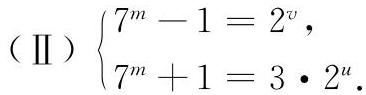
\includegraphics[max width=\textwidth, center]{2024_10_09_7e48ff928cc374c97394g-120}

对(II)中 $7^{m}+1=3 \cdot 2^{u}$ 两边模 3 可得矛盾. \\
对(I )中 $7^{m}+1=2^{v}$ 讨论, 可知 $v \geqslant 3$ , 两边模 8 知 $m$ 为奇数. \\
若 $m=1$ , 则 $v=3$ , 进而由

得\\
故
\begin{align*}
	\begin{gathered}
		7^{m}-1=3 \cdot 2^{u} \\
		u=1 \\
		y=u+v=4
	\end{gathered}
\end{align*}

若 $m>1$ , 则
\begin{align*}
	7^{m}+1=8 \cdot\left(7^{m-1}-7^{m-2}+\cdots-7+1\right)
\end{align*}

其中 $7^{m-1}-7^{m-2}+\cdots-7+1$ 是奇数个奇数之和, 与 $7^{m}+1=2^{u}$ 矛盾.\\
综上, 满足条件的 $(x, y)=(1,1),(2,4)$ . \\
22. 有两种情形, 即
\begin{align*}
	3^{a}-2^{b}=41 \text {, 或 } 2^{b}-3^{a}=41 \text {. }
\end{align*}

对后者可知 $b>3$ , 两边模 8 , 要
\begin{align*}
	3^{a} \equiv 7(\bmod 8)
\end{align*}

但对任意非负整数 $a$ , 有
\begin{align*}
	3^{a} \equiv 1 \text { 或 } 3(\bmod 8),
\end{align*}

矛盾.\\
现在只需讨论 $3^{a}-2^{b}=41$ 的情形. \\
此时, 对等式两边模 3 , 知
\begin{align*}
	2^{b} \equiv 1(\bmod 3)
\end{align*}

故 $b$ 为偶数, 又显然 $b \neq 0$ , 可设 $b=2 n, n$ 为正整数. \\
对等式两边模 4 , 得
\begin{align*}
	3^{a} \equiv 1(\bmod 4)
\end{align*}

故 $a$ 为偶数,设 $a=2 m$ , 就有

故
\begin{align*}
	\begin{gathered}
		\left(3^{m}-2^{n}\right)\left(3^{m}+2^{n}\right)=41 \\
		\left(3^{m}-2^{n}, 3^{m}+2^{n}\right)=(1,41)
	\end{gathered}
\end{align*}

这导致 $2 \cdot 3^{m}=42$ , 即 $3^{m}=21$ , 矛盾. \\
所以, 不存在符合要求的非负整数 $a ,  b$.\\
23. 注意到
\begin{align*}
	36^{k}-5^{m} \equiv \pm 1(\bmod 6)
\end{align*}

故 $36^{k}-5^{m}$ 可能取到的正整数从小到大依次为 $1,11, \cdots$ . \\
现在若 $36^{k}-5^{m}=1$ , 则 $k>1$ , 故两边模 8 , 要求
\begin{align*}
	5^{m} \equiv-1(\bmod 8)
\end{align*}

但 $5^{m} \equiv 1$ 或 $5(\bmod 8) , $ 矛盾.\\
另外, 当 $k=1, m=2$ 时,  $36^{k}-5^{m}=11$ . 所以,  $36^{k}-5^{m}$ 所能取到的最小正整数为 11 .

现在考虑 $5^{m}-36^{k}$ 所能取到的最小正整数, 由\begin{align}
	 & 5^{m}-36^{k} \equiv 4(\bmod 5)     \\
	 & 5^{m}-36^{k} \equiv \pm 1(\bmod 6)
\end{align}

可知
\begin{align*}
	5^{m}-36^{k} \geqslant 19
\end{align*}

综上可知,  $\left|36^{k}-5^{m}\right|$ 的最小可能值为 11.\\
24. 对方程两边模 3 , 可知 $z$ 为偶数, 所以 $3^{x}+2^{2 y}$ 是一个完全平方数. 这样, 利用 3.2 节例 11 的结论, 可知 $x=y=z=2$ . \\
25. 由条件, 知 $x^{2}+y^{2}=z^{2}$ 且 $x+z=2 y$, 则
\begin{align*}
	y^{2}=(z-x)(z+x)=2 y(z-x)
\end{align*}

即
\begin{align*}
	y=2(z-x)
\end{align*}

于是 $y$ 为偶数, 设 $y=2 m$ , 则

解得
\begin{align*}
	\begin{gathered}
		x+z=4 m, z-x=m \\
		x=\frac{3 m}{2}, z=\frac{5 m}{2}
	\end{gathered}
\end{align*}

故 $m$ 为偶数. 因此
\begin{align*}
	(x, y, z)=(3 n, 4 n, 5 n)
\end{align*}

这里 $n=\frac{m}{2}$ 为正整数.\\
26. 因为 $A E \cdot B E=D E \cdot E G$ , 而 $E G=E F+F G=A E+D E$ (用到 $D G / /$ $B C)$ , 故
\begin{align*}
	x(86-x)=y(x+y)
\end{align*}

对等式中的 $x ,  y$ 作奇偶分析, 可知 $x ,  y$ 都为偶数.

将它变形为 $\left(x+\frac{y}{2}-43\right)^{2}+y^{2}=\left(43-\frac{y}{2}\right)^{2}$,\\
故存在正整数 $a ,  b ,  k$, 使得
\begin{align*}
	y=2 a b k, 43-\frac{y}{2}=\left(a^{2}+b^{2}\right) k
\end{align*}

所以
\begin{align*}
	\left(a^{2}+a b+b^{2}\right) k=43,
\end{align*}

于是
\begin{align*}
	k=1,(a, b)=(6,1),(1,6) .
\end{align*}

从而 $y=12$ (此时 $x=2$ 或者 72).\\
27. 只需考虑素数的幂的形式的数 $n$. 为此, 取素数 $p$, 使 $p \equiv 3(\bmod 4)$ (例如 $7,11,19 \cdots)$, 考虑数 $p^{2012}$ .

利用 3.3 节例 2 中的方法, 可知数 $p^{2012}$ 不会是勾股三角形的斜边长.下证: 不定方程 $x^{2}+p^{4024}=z^{2}$ 恰有 2012 组解. 事实上, 因为
\begin{align*}
	(z-x)(z+x)=p^{4024}
\end{align*}

故 $(z-x, z+x)=\left(1, p^{4024}\right),\left(p, p^{4023}\right), \cdots,\left(p^{2011}, p^{2013}\right)$,\\
结合 $p$ 为奇数, 可知求出的每一组 $(x, z)$ 都是正整数, 故 $p^{2012}$ 恰在 2012 组勾股数中出现.

说明 此题的构造方法是基于因式分解, 且由此方法可证: 对任意正整数 $k$, 都有无穷多个正整数 $n$, 数 $n$ 恰好在 $k$ 组勾股数中出现.\\
28. 等价于求满足条件
\begin{align*}
	x+y+z=x y
\end{align*}

的勾股数组 $(x, y, z)$.\\
注意到 $z=\sqrt{x^{2}+y^{2}}$, 于是(1)变为
\begin{align*}
	x^{2}+y^{2}=(x y-x-y)^{2},
\end{align*}

即
\begin{align*}
	x^{2}+y^{2}=x^{2} y^{2}-2 x y(x+y)+x^{2}+2 x y+y^{2},
\end{align*}

故
\begin{align*}
	x^{2} y^{2}-2 x y(x+y)+2 x y=0,
\end{align*}

从而
\begin{align*}
	x y-2(x+y)+2=0
\end{align*}

即
\begin{align*}
	(x-2)(y-2)=2,
\end{align*}

得
\begin{align*}
	(x, y)=(3,4),(4,3)
\end{align*}

综上, 所求直角三角形的三边长为 $3,4,5$.\\
29. 根据 3.3 节开始的分析, 注意到, 勾股三角形的面积还可以表示为\\
$k^{2} m n\left(n^{2}-m^{2}\right)$ 的形式, 其中 $k ,  m ,  n$ 为正整数,  $(m, n)=1, m<n, m$ 与 $n$一奇一偶. 于是 $k^{2} m n\left(n^{2}-m^{2}\right)=24=2^{3} \times 3$ , 故 $k=1$ 或 2 . 若 $k=1$ , 则由 $m ,  n$ 一奇一偶可知 $m ,  n$ 中有一个为 8 的倍数, 这导致 $k^{2} m n\left(m^{2}-n^{2}\right) \geqslant 8 \times$ $3 \times\left(8^{2}-3^{3}\right)>24$ , 故 $k=2$ . 此时 $m n\left(n^{2}-m^{2}\right)=2 \times 3$ , 只能是 $(n, m)=$ $(2,1)$. 故满足条件的三角形只有一个,其边长为 $(6,8,10)$.\\
30. 设 $\triangle A B C$ 各顶点的对应边长为 $a ,  b ,  c$. 过 $A$ 作 $\angle A$ 的平分线交 $B C$于点 $D$, 则
\begin{align*}
	C D=\frac{a b}{b+c}
\end{align*}

利用 $\triangle A C D \backsim \triangle B C A , $ 可知
\begin{align*}
	\frac{C D}{b}=\frac{b}{a}
\end{align*}

即
\begin{align*}
	a^{2}=b(b+c)
\end{align*}

而
\begin{align*}
	\angle C>90^{\circ}
\end{align*}

故
\begin{align*}
	c^{2}>a^{2}+b^{2}
\end{align*}

由
\begin{align*}
	a^{2}=b(b+c)
\end{align*}

设
\begin{align*}
	(b, b+c)=d
\end{align*}

则 $(b, c)=d$ , 并且 $d^{2} \mid a^{2}$ , 故 $d \mid a$ . \\
为求 $a+b+c$ 的最小值, 可设 $d=1$, 这时, $b$ 与 $b+c$ 都为完全平方数,\\
设
\begin{align*}
	b=m^{2}, b+c=n^{2}, m, n \in \mathbf{N}^{*}
\end{align*}

则 $a=m n$ . 利用 $a+b>c$ 及 $c^{2}>a^{2}+b^{2} , $ 可知
\begin{align*}
	m n+m^{2}>n^{2}-m^{2}
\end{align*}

且
\begin{align*}
	\left(n^{2}-m^{2}\right)^{2}>(m n)^{2}+m^{4}
\end{align*}

于是
\begin{align*}
	m>n-m
\end{align*}

即
\begin{align*}
	n<2 m
\end{align*}

并且
\begin{align*}
	n^{4}>3 m^{2} n^{2}
\end{align*}

即
\begin{align*}
	n^{2}>3 m^{2}
\end{align*}

所以
\begin{align*}
	3 m^{2}<n^{2}<4 m^{2}
\end{align*}

从而在 $3 m^{2}$ 与 $4 m^{2}$ 之间有一个完全平方数, 这要求 $m \geqslant 4$, 这时 $n \geqslant 7$,

故
\begin{align*}
	a+b+c \geqslant 4 \times 7+7^{2}=77
\end{align*}

显然 $(a, b, c)=(28,16,33)$ 满足条件, 故所求 $\triangle A B C$ 周长的最小值为 77 . \\
31. 设整数 $a ,  b$ 满足 $5 a \geqslant 7 b \geqslant 0$. 令
\begin{align*}
	w=\left[\frac{b}{5}\right]\left(\text { 表示不超过 } \frac{b}{5} \text { 的最大整数) }, v=b-5 w,\right.
\end{align*}

则当 $v=0,1,2,3,4$ 时( $v$ 只有这 5 种取值), 将原方程组视为关于 $x ,  y ,  z$的不定方程组分别有非负整数解\begin{align}
	  & (x, y, z)                                 \\
	= & (a-7 w, 0,0),(a-7 w-2,1,0),(a-7 w-3,0,1), \\
	  & (a-7 w-5,1,1),(a-7 w-6,0,2) .
\end{align}

所以, 命题成立.\\
32. 当 $n>2 a b c-a b-b c-c a$ 时, 考虑不定方程
\begin{align*}
	x b c+y c a+z a b=n
\end{align*}

的整数解 $(x, y, z)$.
\begin{align*}
	\text { 令 } t=x b+y a, \text { 则 }(z, t) \text { 是方程 }
\end{align*}
\begin{align*}
	c t+z a b=n
\end{align*}

的整数解, 故可设 $0 \leqslant z<c$ (注意, 这里用到 $(c, a b)=1$ 时 (2) 有解), 这时由 (2)知\begin{align}
	t & =\frac{n-z a b}{c}             \\
	  & \geqslant \frac{n-a b(c-1)}{c} \\
	  & >\frac{a b c-b c-c a}{c}       \\
	  & =a b-b-a
\end{align}

而由 3.1 节例 3 的结论, 知 $x b+y a=t$ 有非负整数解. 所以, 此时(1)有非负整数解.

下证: 当 $n=2 a b c-a b-b c-c a$ 时, (1)没有非负整数解.\\
事实上,若存在非负整数组 $(x, y, z)$ 满足
\begin{align*}
	x b c+y c a+z a b=2 a b c-a b-b c-c a
\end{align*}

则
\begin{align*}
	(x+1) b c+(y+1) c a+(z+1) a b=2 a b c
\end{align*}

利用 $a ,  b ,  c$ 两两互素, 可知

导致
\begin{align*}
	a|x+1, b| y+1, c \mid z+1
\end{align*}\begin{align}
	2 a b c & =(x+1) b c+(y+1) c a+(z+1) a b      \\
	        & \geqslant a b c+b c a+c a b=3 a b c
\end{align}

矛盾. 所以命题成立.\\
33. 设 $n$ 是一个满足条件的数, 则 $n>1$, 且此时只有一个数 (即 1 ) 既是 $n$的因数, 又是与 $n$ 互素的数. 故 $1,2, \cdots, n$ 中恰好有一个数, 它既不是 $n$ 的因数, 又不与 $n$ 互素.

由于 $n>1$ 时, $\varphi(n)$ 为偶数, 若 $n$ 为偶数, 则在 $n \geqslant 10$ 时, 数 $n-2$ 与 $n-4$既不与 $n$ 互素, 又不是 $n$ 的因数, 故 $n \geqslant 10$ 且 $n$ 为偶数时, $n$ 不满足条件; 若 $n$为奇数, 则 $d(n)$ 为奇数, 此时 $n$ 是一个完全平方数. 设 $n=(2 m+1)^{2}$, 若 $m>1$, 则数 $n-(2 m+1)$ 和 $n-2(2 m+1)$ 都不是 $n$ 的因数, 且都不与 $n$ 互素, 此时, $n$ 不满足条件.

综上, 只需对 $n=2,4,6,8,9$ 进行验算, 可知满足条件的 $n=6,8,9$.\\
34. 我们利用勾股数来构造. 任取一组勾股数 $(x, y, z)$ (不必是本原的),令
\begin{align*}
	a=x\left|4 y^{2}-z^{2}\right|, b=y\left|4 x^{2}-z^{2}\right|, c=4 x y z
\end{align*}

则有\begin{align}
	a^{2}+b^{2} & =x^{2}\left(3 y^{2}-x^{2}\right)^{2}+y^{2}\left(3 x^{2}-y^{2}\right)^{2} \\
	            & =x^{6}+3 x^{2} y^{4}+3 x^{4} y^{2}+y^{6}                                 \\
	            & =\left(x^{2}+y^{2}\right)^{3}=\left(z^{3}\right)^{2}                     \\
	            & a^{2}+c^{2}=x^{2}\left(4 y^{2}+z^{2}\right)^{2}                          \\
	            & b^{2}+c^{2}=y^{2}\left(4 x^{2}+z^{2}\right)^{2}
\end{align}

由于勾股数有无穷多组, 从而符合条件的三元正整数数组有无穷多组.\\
例如: 当 $x=3, y=4, z=5$ 时, 得出
\begin{align*}
	a=117, b=44, c=240
\end{align*}

并且
\begin{align*}
	117^{2}+44^{2}=125^{2}, 117^{2}+240^{2}=267^{2}, 44^{2}+240^{2}=244^{2}
\end{align*}\\
35. 两边模 11, 由 Fermat 小定理知, 当 $11 \nmid y$ 时, 有
\begin{align*}
	y^{10} \equiv 1(\bmod 11)
\end{align*}

故此时\\
所以总有\\
即\\
另一方面, 对 $x^{2}$ 而言, 由于
\begin{align*}
	x \equiv 0, \pm 1, \pm 2, \pm 3, \pm 4, \pm 5(\bmod 11)
\end{align*}

故
\begin{align*}
	x^{2} \equiv 0,1,4,9,5,3(\bmod 11)
\end{align*}

所以,  $x^{2}=y^{5}-4$ 没有整数解. \\
36. 两边模 13 去处理. 由 Fermat 小定理知, 当 $13 \nmid m$ 时,有 $m^{12} \equiv 1(\bmod 13)$ , 得 $m^{6} \equiv 1$ 或 $25(\bmod 13)$ , 所以,  $m^{3} \equiv \pm 1$ 或 $\pm 5(\bmod 13)$ , 即总有 $m^{3} \equiv 0,1$ ,  $5,8,12(\bmod 13)$.

与上题类似, 可知 $n^{2} \equiv 0,1,4,9,3,12(\bmod 13)$ , 于是,  $n^{4} \equiv 0,1,3$ 或 $9(\bmod 13)$ .

利用上述结论, 可知, 对正整数 $m ,  n$ , 总有
\begin{align*}
	m^{3}+n^{4} \equiv 0,1,2,3,4,5,6,8,9,10,11,12(\bmod 13)
\end{align*}

即 $m^{3}+n^{4} \not \equiv 7(\bmod 13)$.\\
然而,  $19^{19} \equiv 6^{19} \equiv 6^{7} \equiv-6 \equiv 7(\bmod 13)$ (这里用到 Fermat 小定理及 $\left.6^{6} \equiv-1(\bmod 13)\right)$.

所以, 不存在使 $19^{19}=m^{3}+n^{4}$ 成立的正整数 $m ,  n$ . \\
说明 上述两题中模参数的选择是基于 Fermat 小定理的反用(第 35 题中,  2,5 都是 $11-1$ 的因数, 而第 36 题中,  3,4 都是 $13-1$ 的因数), 此时所涉幂次对模参数所得的余数相对容易控制, 从而能一步到位导出矛盾. \\
37. 注意到 $(x, y, z, u, v)=(1,2,3,4,5)$ 是原方程的正整数解.

一般地, 设 $(x, y, z, u, v)$ 是原方程的正整数解, 且 $x<y<z<u<v , $则将原方程视为关于 $x$ 的一元二次方程, 利用韦达定理可知( $y z u v-x, y$ ,  $z, u, v)$ 也是原方程的正整数解, 依对称性, 可知 $(y, z, u, v, y z u v-x)$ 也是解, 并且满足条件 $y<z<u<v<y z u v-x$ . 依此递推方式, 可得原方程的无穷多组正整数解, 并且后一步构造的解中, 最小的数比前一组解中最小的数大.

所以, 存在满足条件的正整数解. \\
38. 分别就 $a$ 的不同情况讨论方程
\begin{align*}
	x^{2}+a x y+y^{2}=1
\end{align*}

的整数解的组数.\\
当 $a=0$ 时, 方程为 $x^{2}+y^{2}=1$, 仅有 4 组整数解.\\
若 $a \neq 0$, 则 $(x, y)$ 为方程 (1) 的解的充要条件是: $(x,-y)$ 为方程 $x^{2}-$ $a x y+y^{2}=1$ 的解. 所以, 只需讨论 $a<0$ 且方程 (1) 有无穷多组非负整数解 $(x, y)$ 的情形.

若 $a=-1$, 则 (1) 为 $x^{2}-x y+y^{2}=1$, 两边乘以 4 , 再配方得 $(2 x-y)^{2}+$ $3 y^{2}=4$ , 仅有两组非负整数解.

如果 $a<-1$, 那么 $(-a, 1)$ 为(1)的一组正整数解. 一般地, 设 $(x, y)$ 为(1)的正整数解, 且 $x>y$, 则 $(x,-a x+y)$ 也是(1)的解 (这一个解, 在视(1)为关于 $y$ 的一元二次方程时, 利用韦达定理可得), 当然 ( $-a x+y, x$ )(满足 $-a x+y>x>y)$ 也是(1)的正整数解, 依此递推, 可知这时(1)有无穷多组正整数解.

综上所述,当 $|a|>1$ 时, 方程(1)有无穷多组整数解,而 $|a| \leqslant 1$ 时, (1)仅有有限组整数解.\\
39. 由条件可知 $x \geqslant 2$.

如果 $n$ 为偶数, 那么由完全平方数 $\equiv 0$ 或 $1(\bmod 3)$ 可知 $x^{n} \equiv 0$ 或 $1(\bmod 3)$ , 但 $3^{k}-1 \equiv 2(\bmod 3)$ , 此时无解.

如果 $n$ 为奇数, 那么
\begin{align*}
	3^{k}=x^{n}-1=(x+1)\left(x^{n-1}-x^{n-2}+\cdots-x+1\right) .
\end{align*}

所以,  $x+1$ 和 $A=x^{n-1}-x^{n-2}+\cdots-x+1$ 都为 3 的幂次. \\
注意到,
\begin{align*}
	A \equiv(-1)^{n-1}-(-1)^{n-2}+\cdots-(-1)+1=n(\bmod (x+1))
\end{align*}

故 $n$ 为 3 的倍数. 可设 $n=3 m$, 记 $y=x^{m}$, 则
\begin{align*}
	3^{k}=y^{3}+1=(y+1)\left(y^{2}-y+1\right)
\end{align*}

从而, $y+1$ 和 $y^{2}-y+1$ 都是 3 的幂次.\\
设 $y+1=3^{t}$ , 则由(1)知
\begin{align*}
	3^{k}=\left(3^{t}-1\right)^{3}+1=3^{3 t}-3^{2 t+1}+3^{t+1} .
\end{align*}

如果 $t>1$, 那么 $3 t>2 t+1>t+1$, 此时 $3^{t+1} \| 3^{3 t}-3^{2 t+1}+3^{t+1}$, 对比 (2) 式两边要求 $k=t+1$, 但此时 (2) 的左边小于右边. 所以, $t=1$, 进而, $y=2, k=2$.得 $(x, k, n)=(2,2,3)$.

综上可知, 符合条件的正整数 $(x, k, n)=(2,2,3)$.\\
40. 记 $F(x, y)=x^{3}-x^{2} y+y^{2}+x-y$, 则 $F(1,1)=1, F(1,2)=2$.

因此, $n=1,2$ 时, 方程有正整数解.\\
下证:  $F(x, y)=3$ 没有正整数解. \\
视方程 $F(x, y)=3$ 为关于 $y$ 的一元二次方程
\begin{align*}
	y^{2}-\left(x^{2}+1\right) y+x^{3}+x-3=0
\end{align*}

如果存在正整数解, 那么
\begin{align*}
	\Delta=\left(x^{2}+1\right)^{2}-4\left(x^{3}+x-3\right)=x^{4}-4 x^{3}+2 x^{2}-4 x+13
\end{align*}

\section{是一个完全平方数.}
注意到, 当 $x \geqslant 2$ 时, 有 $\Delta<\left(x^{2}-2 x-1\right)^{2}$ , 而 $x \geqslant 6$ 时, 有 $\Delta>\left(x^{2}-\right.$ $2 x-2)^{2}$, 故 $x \geqslant 6$ 时, $\Delta$ 不是完全平方数. 而当 $x=1,2,3,4,5$ 时, 对应的 $\Delta=8,-3,-8,29,168$ 都不是完全平方数, 故 $n=3$ 时无正整数解.

综上可知, 所求的最小正整数 $n=3$.






